

\chapter{Results and Evaluation}
\section{Results for Workload A}
\subsection{Comparing Existing Work: Virtual Machine vs the Reference Value}
\subsubsection{Initial Observations}
The result medians are displayed in Figure \ref{figures-wla_fig5}.  As expected, the virtual machine results imply much, much less execution time compared to the reference value, presumably accounting for diminished network latency. Such network latency seems to have an increasing effect on the reference as the cluster size goes up, but further analysis would be required to even make this claim. \begin{figure}[h]
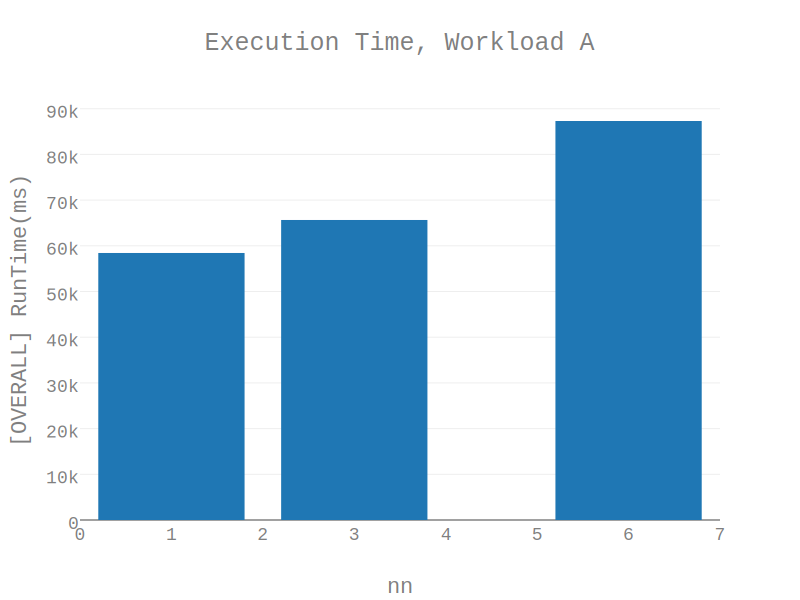
\includegraphics[width=5.5in]{Figures/figures-wla_fig1.pdf}
\caption{}
\label{figures-wla_fig1}
\end{figure}

\begin{figure}[h]
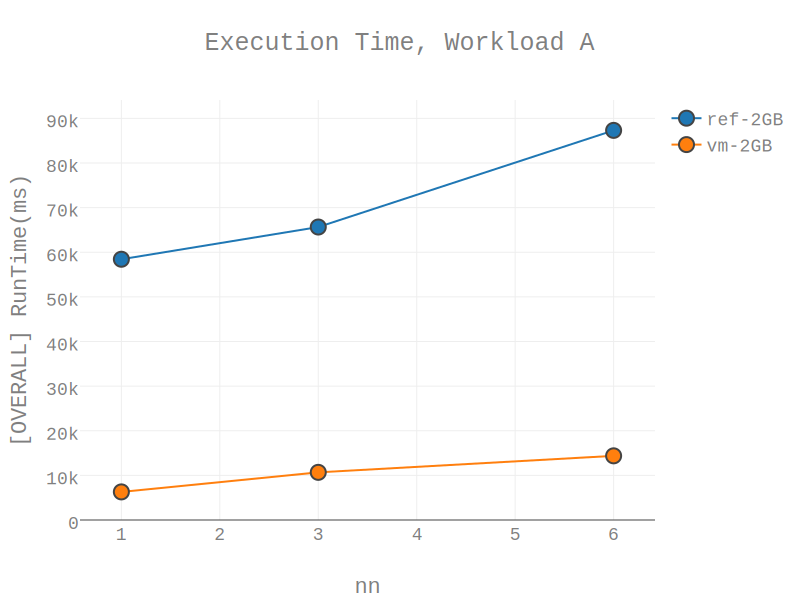
\includegraphics[width=5.5in]{Figures/figures-wla_fig5.pdf}
\caption{}
\label{figures-wla_fig5}
\end{figure}



\subsubsection{Ordinal Statistics}
This section will describe some of the summary statistics that describe the data.  

The summary statistics for Workload A performed on the virtual machines are in Tables \ref{table:summary_table_a_1GB_vm_nodal}, \ref{table:summary_table_a_2GB_vm_nodal}, and \ref{table:summary_table_a_4GB_vm_nodal}.
\begin{table}
\begin{tabular}{lrrrr}
\toprule
cluster\_size &     1.0 &     3.0 &     6.0 &  Overall \\
\midrule
25\%   & 6.2e+03 &   1e+04 & 1.4e+04 &  6.3e+03 \\
50\%   & 6.3e+03 &   1e+04 & 1.4e+04 &    1e+04 \\
75\%   & 6.3e+03 & 1.1e+04 & 1.4e+04 &  1.4e+04 \\
count &      21 &      21 &      21 &       63 \\
max   & 6.3e+03 & 1.1e+04 & 1.5e+04 &  1.5e+04 \\
mean  & 6.2e+03 & 1.1e+04 & 1.4e+04 &    1e+04 \\
min   & 6.1e+03 &   1e+04 & 1.4e+04 &  6.1e+03 \\
range & 2.8e+02 & 6.8e+02 & 6.8e+02 &  8.6e+03 \\
std   &      84 & 2.2e+02 & 1.7e+02 &  3.3e+03 \\
\bottomrule
\end{tabular}
\caption{Summary Statistics for Workload A performed on a 2GB virtual machine node over a(n)nodal network.  Except for count, all values are in milliseconds.}
\label{table:summary_table_a_2GB_vm_nodal}
\end{table}



\subsubsection{Analysis}
This section will take a more in-depth look at the data.
:::something went wrong generating the speedup analysis tables:::

\subsection{1GB RAM vs 2GB RAM vs 4GB RAM}
\subsubsection{Initial Observations}
This section discusses testing and performance for memory sizes: 1GB, 2GB, and 4GB.  The results are displayed in Figure \ref{figures-wla_fig4}. While it appears the varying the amount of memory has some effect on the results, theredoes not seem to be a predictable pattern across nodes. An ANOVA test will determine if there is an effect, and a linear regression will further testfor an effect. \begin{figure}[h]
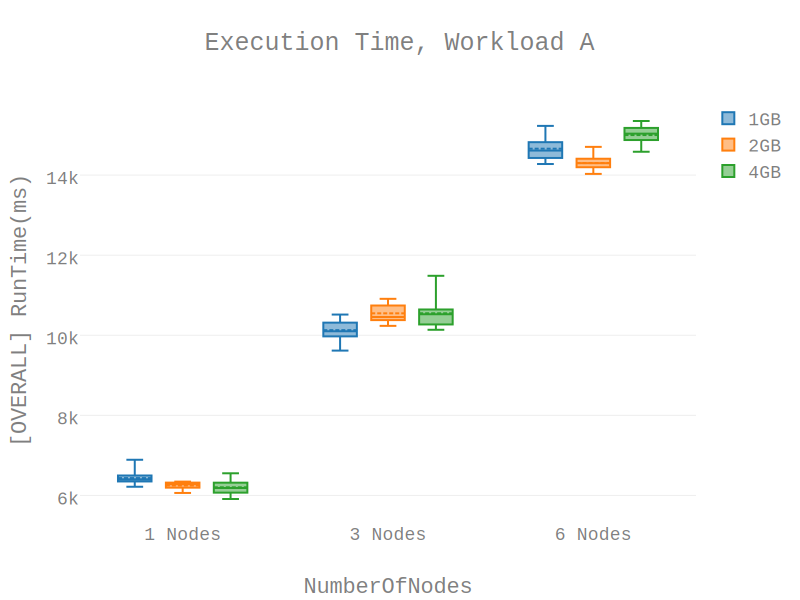
\includegraphics[width=5.5in]{Figures/figures-wla_fig4.pdf}
\caption{}
\label{figures-wla_fig4}
\end{figure}



\subsubsection{Ordinal Statistics}
This section will describe some of the summary statistics that describe the data.  

The summary statistics for Workload A performed on the virtual machines are in Tables \ref{table:summary_table_a_1GB_vm_nodal}, \ref{table:summary_table_a_2GB_vm_nodal}, and \ref{table:summary_table_a_4GB_vm_nodal}.
\begin{table}
\begin{tabular}{lrrrr}
\toprule
cluster\_size &     1.0 &     3.0 &     6.0 &  Overall \\
\midrule
25\%   & 6.4e+03 &   1e+04 & 1.4e+04 &  6.5e+03 \\
50\%   & 6.4e+03 &   1e+04 & 1.5e+04 &    1e+04 \\
75\%   & 6.5e+03 &   1e+04 & 1.5e+04 &  1.4e+04 \\
count &      21 &      21 &      21 &       63 \\
max   & 6.9e+03 & 1.1e+04 & 1.5e+04 &  1.5e+04 \\
mean  & 6.4e+03 &   1e+04 & 1.5e+04 &    1e+04 \\
min   & 6.2e+03 & 9.6e+03 & 1.4e+04 &  6.2e+03 \\
range & 6.7e+02 &   9e+02 & 9.5e+02 &    9e+03 \\
std   & 1.4e+02 & 2.3e+02 & 2.7e+02 &  3.4e+03 \\
\bottomrule
\end{tabular}
\caption{Summary Statistics for Workload A performed on a 1GB virtual machine node over a(n)nodal network.  Except for count, all values are in milliseconds.}
\label{table:summary_table_a_1GB_vm_nodal}
\end{table}

\begin{table}
\begin{tabular}{lrrrr}
\toprule
cluster\_size &     1.0 &     3.0 &     6.0 &  Overall \\
\midrule
25\%   & 6.1e+03 &   1e+04 & 1.5e+04 &  6.3e+03 \\
50\%   & 6.2e+03 & 1.1e+04 & 1.5e+04 &  1.1e+04 \\
75\%   & 6.3e+03 & 1.1e+04 & 1.5e+04 &  1.5e+04 \\
count &      21 &      21 &      21 &       63 \\
max   & 6.6e+03 & 1.1e+04 & 1.5e+04 &  1.5e+04 \\
mean  & 6.2e+03 & 1.1e+04 & 1.5e+04 &  1.1e+04 \\
min   & 5.9e+03 &   1e+04 & 1.5e+04 &  5.9e+03 \\
range & 6.4e+02 & 1.3e+03 & 7.7e+02 &  9.4e+03 \\
std   & 1.7e+02 & 3.4e+02 & 2.2e+02 &  3.6e+03 \\
\bottomrule
\end{tabular}
\caption{Summary Statistics for Workload A performed on a 4GB virtual machine node over a(n)nodal network.  Except for count, all values are in milliseconds.}
\label{table:summary_table_a_4GB_vm_nodal}
\end{table}




\subsubsection{Analysis}
This section will take a more in-depth look at the data.


\begin{table}[H]
\centering
\begin{tabular}{rrrrrr}
\toprule
 cluster\_size &   slope &  intercept &  r\_value &  p\_value &  std\_err \\
\midrule
            1 &     -69 &    6.5e+03 &    -0.51 &  2.1e-05 &       15 \\
            3 & 1.2e+02 &      1e+04 &     0.46 &  0.00016 &       30 \\
            6 & 1.5e+02 &    1.4e+04 &     0.51 &  1.7e-05 &       32 \\
\bottomrule
\end{tabular}
\caption{Linear Regression over amount of RAM}
\label{table:ram_v_ram_a}
\end{table}



\subsection{Implementation on Raspberry Pi}
\subsubsection{Initial Observations}
The results are displayed in Figure \ref{figures-wla_fig10}.  \begin{figure}[h]
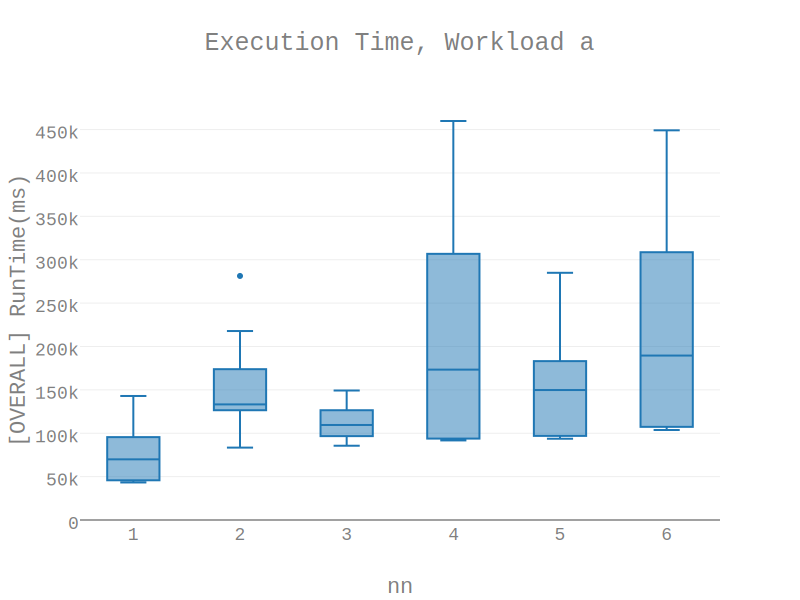
\includegraphics[width=5.5in]{Figures/figures-wla_fig10.pdf}
\caption{}
\label{figures-wla_fig10}
\end{figure}



\subsubsection{Ordinal Statistics}
This section will describe some of the summary statistics that describe the data.  

The summary statistics for Workload A performed on the limited hardware, Raspberry Pi, on the Ethernet local area network are in Table \ref{table:summary_table_a_1GB_rp_eth}.
\begin{table}
\begin{tabular}{lrrrrrrr}
\toprule
cluster\_size &     1.0 &     2.0 &     3.0 &     4.0 &     5.0 &     6.0 &  Overall \\
\midrule
25\%   & 4.5e+04 & 1.3e+05 & 9.6e+04 & 9.4e+04 & 9.6e+04 & 1.1e+05 &  9.4e+04 \\
50\%   & 4.6e+04 & 1.3e+05 & 9.7e+04 & 9.4e+04 & 9.6e+04 & 1.1e+05 &  9.7e+04 \\
75\%   & 4.6e+04 & 1.3e+05 & 9.8e+04 & 9.5e+04 & 9.8e+04 & 1.1e+05 &  1.1e+05 \\
count &      21 &      21 &      21 &      21 &      21 &      21 &  1.3e+02 \\
max   & 4.8e+04 & 1.3e+05 &   1e+05 & 9.6e+04 & 9.9e+04 & 1.1e+05 &  1.3e+05 \\
mean  & 4.6e+04 & 1.3e+05 & 9.7e+04 & 9.4e+04 & 9.6e+04 & 1.1e+05 &  9.5e+04 \\
min   & 4.3e+04 & 1.2e+05 & 9.4e+04 & 9.3e+04 & 9.4e+04 &   1e+05 &  4.3e+04 \\
range & 4.9e+03 & 1.5e+04 & 6.8e+03 & 3.6e+03 & 4.9e+03 & 7.3e+03 &  8.8e+04 \\
std   & 1.1e+03 & 3.5e+03 & 1.6e+03 & 9.2e+02 & 1.5e+03 & 1.8e+03 &  2.5e+04 \\
\bottomrule
\end{tabular}
\caption{Summary Statistics for Workload A performed on a 1GB limited hardware, Raspberry Pi node over a(n)Ethernet network.  Except for count, all values are in milliseconds.}
\label{table:summary_table_a_1GB_rp_eth}
\end{table}



\subsubsection{Analysis}
This section will take a more in-depth look at the data.


\begin{table}[H]
\centering
\begin{tabular}{rrrrr}
\toprule
 slope &  intercept &  r\_value &  p\_value &  std\_err \\
\midrule
 6e+03 &    7.3e+04 &     0.42 &  1.1e-06 &  1.2e+03 \\
\bottomrule
\end{tabular}
\caption{Linear Regression over Cluster Size, Workload a}
\label{table:rp_only_a}
\end{table}



\subsection{Raspberry Pi vs Reference Value}
\subsubsection{Initial Observations}
The results are displayed in Figure \ref{figures-wla_fig6}.  The performance of the limited hardware, the Raspberry Pi, seems comparable with the results from the more appropriate in the other paper.  In addition, there is no reason to suspect a significant differential in the overall pattern with respect to scalability: performance over cluster size. \begin{figure}[h]
\includegraphics[width=5.5in]{Figures/figures-wla_fig6.pdf}
\caption{}
\label{figures-wla_fig6}
\end{figure}



\subsubsection{Ordinal Statistics}
This section will describe some of the summary statistics that describe the data.  

The summary statistics for Workload A performed on the limited hardware, Raspberry Pi, on the Ethernet local area network are in Table \ref{table:summary_table_a_1GB_rp_eth}.



\subsubsection{Analysis}
This section will take a more in-depth look at the data.
:::something went wrong generating the speedup analysis tables:::

\subsection{Raspberry Pi vs Virtual Machine}
\subsubsection{Initial Observations}
The results are displayed in Figure \ref{figures-wla_fig6}.  As expected, there is a significant differential between the limited hardware, the Raspberry Pi configuration and the virtual machine.  However, it is not clear if this is linear across cluster size. 

\subsubsection{Ordinal Statistics}
This section will describe some of the summary statistics that describe the data.  

The summary statistics for Workload A performed on the virtual machines are in Tables \ref{table:summary_table_a_1GB_vm_nodal}, \ref{table:summary_table_a_2GB_vm_nodal}, and \ref{table:summary_table_a_4GB_vm_nodal}.
The summary statistics for Workload A performed on the limited hardware, Raspberry Pi, on the Ethernet local area network are in Table \ref{table:summary_table_a_1GB_rp_eth}.



\subsubsection{Analysis}
This section will take a more in-depth look at the data.




\begin{table}[H]
\centering
\begin{tabular}{lrrrrr}
\toprule
cluster\_size &   slope &  intercept &  r\_value &  p\_value &  std\_err \\
\midrule
           1 & 3.9e+04 &    6.4e+03 &        1 &  1.3e-57 &  2.5e+02 \\
           2 &     nan &        nan &        0 &        1 &      inf \\
           3 & 8.7e+04 &      1e+04 &        1 &  8.6e-65 &  3.6e+02 \\
           4 &     nan &        nan &        0 &        1 &      inf \\
           5 &     nan &        nan &        0 &        1 &      inf \\
           6 & 9.2e+04 &    1.5e+04 &        1 &  2.3e-64 &  3.9e+02 \\
     OVERALL & 8.4e+04 &      1e+04 &     0.89 &  4.5e-66 &  3.1e+03 \\
\bottomrule
\end{tabular}
\caption{Linear Regression over the effect of limited hardware, Workload A}
\label{table:rp_v_vm_a}
\end{table}





\begin{table}[H]
\centering
\begin{tabular}{llllllll}
\toprule
{} &    0 &    1 &     2 &    3 &    4 &    5 &        6 \\
\midrule
cluster\_size         &    1 &    2 &     3 &    4 &    5 &    6 &  OVERALL \\
ratio\_max\_to\_min     & 0.16 &  NaN &  0.11 &  NaN &  NaN & 0.15 &     0.35 \\
ratio\_min\_to\_max     & 0.13 &  NaN & 0.096 &  NaN &  NaN & 0.13 &    0.047 \\
ratio\_of\_the\_means   & 0.14 &  NaN &   0.1 &  NaN &  NaN & 0.14 &     0.11 \\
ratio\_of\_the\_medians & 0.14 &  NaN &   0.1 &  NaN &  NaN & 0.14 &      0.1 \\
ratio\_of\_the\_stddevs & 0.13 &  NaN &  0.14 &  NaN &  NaN & 0.15 &     0.14 \\
\bottomrule
\end{tabular}
\caption{Speedup over the effect of limited hardware, Workload A}
\label{table:rp_v_vm_a_speedup}
\end{table}





\subsection{Wireless Links Only}
\subsubsection{Initial Observations}
The results are displayed in Figure \ref{figures-wla_fig8}.  Although there is a general trend of increased execution time over cluster size, the oscillation that occurs between odd and even node cluster sizes is hard to miss. This may be result of the collision avoidance strategy, but further experiments would be needed to determine a more specific explanation. \begin{figure}[h]
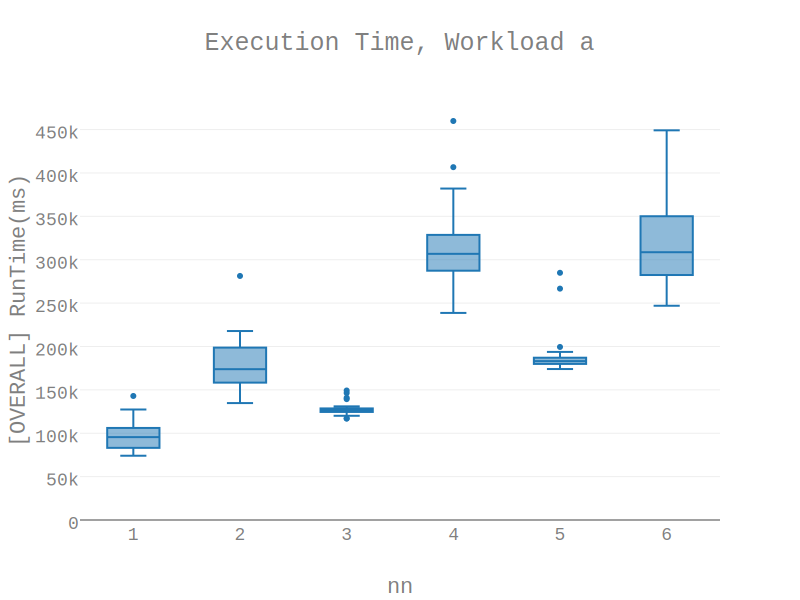
\includegraphics[width=5.5in]{Figures/figures-wla_fig8.pdf}
\caption{}
\label{figures-wla_fig8}
\end{figure}



\subsubsection{Ordinal Statistics}
This section will describe some of the summary statistics that describe the data.  

The summary statistics for Workload A performed on the limited hardware, Raspberry Pi, on the Ethernet local area network are in Table \ref{table:summary_table_a_1GB_rp_wlan}.
\begin{table}
\begin{tabular}{lrrrrrrr}
\toprule
cluster\_size &     1.0 &     2.0 &     3.0 &     4.0 &     5.0 &     6.0 &  Overall \\
\midrule
25\%   & 8.2e+04 & 1.7e+05 & 1.3e+05 &   3e+05 & 1.8e+05 & 2.7e+05 &  1.3e+05 \\
50\%   &   9e+04 & 1.8e+05 & 1.3e+05 & 3.2e+05 & 1.8e+05 &   3e+05 &  1.8e+05 \\
75\%   &   1e+05 &   2e+05 & 1.3e+05 & 3.3e+05 & 1.8e+05 & 3.1e+05 &  2.8e+05 \\
count &      21 &      21 &      21 &      21 &      21 &      21 &  1.3e+02 \\
max   & 1.2e+05 & 2.8e+05 & 1.5e+05 & 4.6e+05 & 2.8e+05 & 3.6e+05 &  4.6e+05 \\
mean  & 9.1e+04 & 1.9e+05 & 1.3e+05 & 3.2e+05 & 1.9e+05 &   3e+05 &    2e+05 \\
min   & 7.4e+04 & 1.5e+05 & 1.2e+05 & 2.6e+05 & 1.7e+05 & 2.5e+05 &  7.4e+04 \\
range & 4.6e+04 & 1.3e+05 & 2.6e+04 & 1.9e+05 & 1.1e+05 & 1.1e+05 &  3.9e+05 \\
std   & 1.3e+04 & 2.9e+04 & 7.4e+03 & 4.5e+04 & 2.9e+04 & 3.2e+04 &  8.7e+04 \\
\bottomrule
\end{tabular}
\caption{Summary Statistics for Workload A performed on a 1GB limited hardware, Raspberry Pi node over a(n)802.11a/b/g/n network.  Except for count, all values are in milliseconds.}
\label{table:summary_table_a_1GB_rp_wlan}
\end{table}



\subsubsection{Analysis}
This section will take a more in-depth look at the data.


\begin{table}[H]
\centering
\begin{tabular}{rrrrr}
\toprule
  slope &  intercept &  r\_value &  p\_value &  std\_err \\
\midrule
3.5e+04 &      8e+04 &     0.69 &  7.5e-19 &  3.3e+03 \\
\bottomrule
\end{tabular}
\caption{Linear Regression over Cluster Size, Workload a}
\label{table:wlan_only_a}
\end{table}



\subsection{Wireless Links vs Wired Links}
\subsubsection{Initial Observations}
The results are displayed in Figures \ref{figures-wla_fig7} and \ref{figures-wla_fig9}.  For 1, 2, and 3-node clusters, despite the expected  disparity in execution time, the wired and wireless trends seem to follow each other.  However, from 3 nodes up through 6 nodes, the execution times starts to diverge, suggesting that the wireless has a increasing effect as the number of nodes increases. \begin{figure}[h]
\includegraphics[width=5.5in]{Figures/figures-wla_fig7.pdf}
\caption{}
\label{figures-wla_fig7}
\end{figure}

\begin{figure}[h]
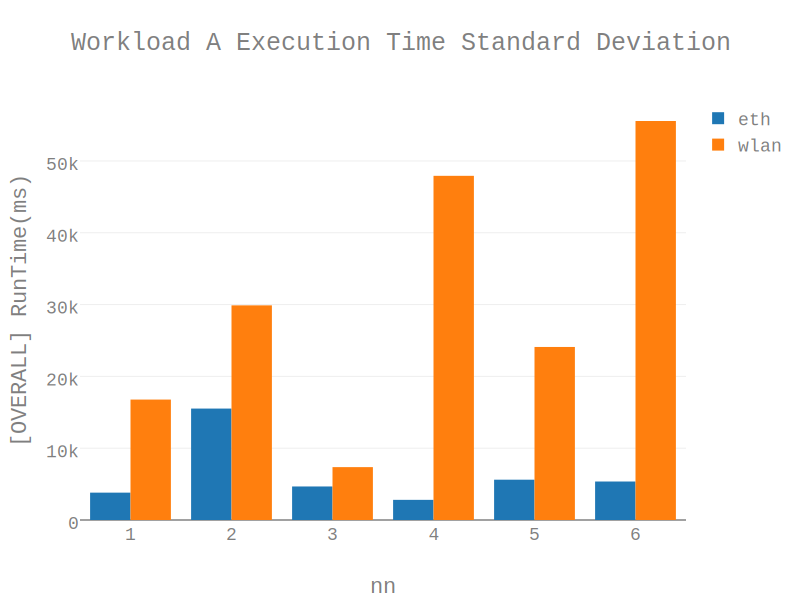
\includegraphics[width=5.5in]{Figures/figures-wla_fig9.pdf}
\caption{}
\label{figures-wla_fig9}
\end{figure}



\subsubsection{Ordinal Statistics}
This section will describe some of the summary statistics that describe the data.  

The summary statistics for Workload A performed on the limited hardware, Raspberry Pi, on the Ethernet local area network are in Table \ref{table:summary_table_a_1GB_rp_eth}.
The summary statistics for Workload A performed on the limited hardware, Raspberry Pi, on the Ethernet local area network are in Table \ref{table:summary_table_a_1GB_rp_wlan}.



\subsubsection{Analysis}
This section will take a more in-depth look at the data.




\begin{table}[H]
\centering
\begin{tabular}{lrrrrr}
\toprule
cluster\_size &   slope &  intercept &  r\_value &  p\_value &  std\_err \\
\midrule
           1 & 4.6e+04 &    4.6e+04 &     0.93 &  3.9e-19 &  2.8e+03 \\
           2 & 6.1e+04 &    1.3e+05 &     0.84 &  3.7e-12 &  6.3e+03 \\
           3 & 3.3e+04 &    9.7e+04 &     0.95 &  2.9e-22 &  1.7e+03 \\
           4 & 2.3e+05 &    9.4e+04 &     0.96 &  9.4e-25 &  9.8e+03 \\
           5 & 9.4e+04 &    9.6e+04 &     0.92 &  4.6e-18 &  6.3e+03 \\
           6 & 1.9e+05 &    1.1e+05 &     0.97 &  1.4e-27 &  6.9e+03 \\
     OVERALL & 1.1e+05 &    9.5e+04 &     0.65 &  3.4e-31 &  8.1e+03 \\
\bottomrule
\end{tabular}
\caption{Linear Regression over the effect of 802.11 links, Workload A}
\label{table:wlan_v_eth_a}
\end{table}





\begin{table}[H]
\centering
\begin{tabular}{llllllll}
\toprule
{} &     0 &    1 &    2 &    3 &     4 &     5 &        6 \\
\midrule
cluster\_size         &     1 &    2 &    3 &    4 &     5 &     6 &  OVERALL \\
ratio\_max\_to\_min     &  0.65 & 0.87 & 0.82 & 0.36 &  0.57 &  0.45 &      1.8 \\
ratio\_min\_to\_max     &  0.36 & 0.42 & 0.63 &  0.2 &  0.33 &  0.29 &    0.094 \\
ratio\_of\_the\_means   &   0.5 & 0.67 & 0.75 & 0.29 &  0.51 &  0.36 &     0.47 \\
ratio\_of\_the\_medians &  0.51 & 0.72 & 0.76 &  0.3 &  0.53 &  0.35 &     0.53 \\
ratio\_of\_the\_stddevs & 0.087 & 0.12 & 0.22 & 0.02 & 0.052 & 0.057 &     0.28 \\
\bottomrule
\end{tabular}
\caption{Speedup over the effect of 802.11 links, Workload A}
\label{table:wlan_v_eth_a_speedup}
\end{table}





\section{Results for Workload C}
\subsection{Comparing Existing Work: Virtual Machine vs the Reference Value}
\subsubsection{Initial Observations}
The result medians are displayed in Figure \ref{figures-wlc_fig5}.  As expected, the virtual machine results imply much, much less execution time compared to the reference value, presumably accounting for diminished network latency. Such network latency seems to have an increasing effect on the reference as the cluster size goes up, but further analysis would be required to even make this claim. \begin{figure}[h]
\includegraphics[width=5.5in]{Figures/figures-wlc_fig1.pdf}
\caption{}
\label{figures-wlc_fig1}
\end{figure}

\begin{figure}[h]
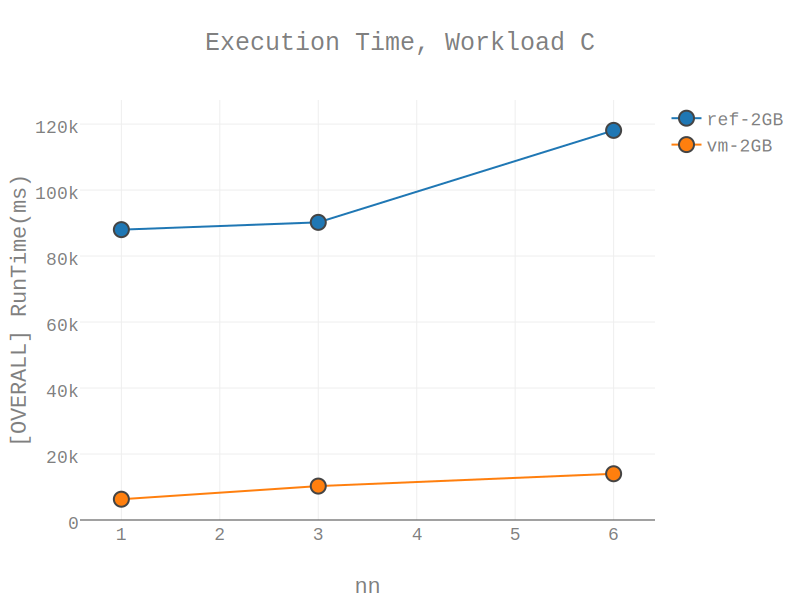
\includegraphics[width=5.5in]{Figures/figures-wlc_fig5.pdf}
\caption{}
\label{figures-wlc_fig5}
\end{figure}



\subsubsection{Ordinal Statistics}
This section will describe some of the summary statistics that describe the data.  

The summary statistics for Workload C performed on the virtual machines are in Tables \ref{table:summary_table_c_1GB_vm_nodal}, \ref{table:summary_table_c_2GB_vm_nodal}, and \ref{table:summary_table_c_4GB_vm_nodal}.
\begin{table}
\begin{tabular}{lrrrr}
\toprule
cluster\_size &     1.0 &     3.0 &     6.0 &  Overall \\
\midrule
25\%   & 6.2e+03 &   1e+04 & 1.4e+04 &  6.3e+03 \\
50\%   & 6.2e+03 &   1e+04 & 1.4e+04 &    1e+04 \\
75\%   & 6.3e+03 &   1e+04 & 1.4e+04 &  1.4e+04 \\
count &      21 &      21 &      21 &       63 \\
max   & 6.9e+03 &   1e+04 & 1.4e+04 &  1.4e+04 \\
mean  & 6.3e+03 &   1e+04 & 1.4e+04 &    1e+04 \\
min   &   6e+03 & 9.8e+03 & 1.3e+04 &    6e+03 \\
range & 9.8e+02 &   6e+02 & 9.8e+02 &  8.5e+03 \\
std   & 2.2e+02 & 1.8e+02 & 2.6e+02 &  3.2e+03 \\
\bottomrule
\end{tabular}
\caption{Summary Statistics for Workload C performed on a 2GB virtual machine node over a(n)nodal network.  Except for count, all values are in milliseconds.}
\label{table:summary_table_c_2GB_vm_nodal}
\end{table}



\subsubsection{Analysis}
This section will take a more in-depth look at the data.
:::something went wrong generating the speedup analysis tables:::

\subsection{1GB RAM vs 2GB RAM vs 4GB RAM}
\subsubsection{Initial Observations}
This section discusses testing and performance for memory sizes: 1GB, 2GB, and 4GB.  The results are displayed in Figure \ref{figures-wlc_fig4}. While it appears the varying the amount of memory has some effect on the results, theredoes not seem to be a predictable pattern across nodes. An ANOVA test will determine if there is an effect, and a linear regression will further testfor an effect. \begin{figure}[h]
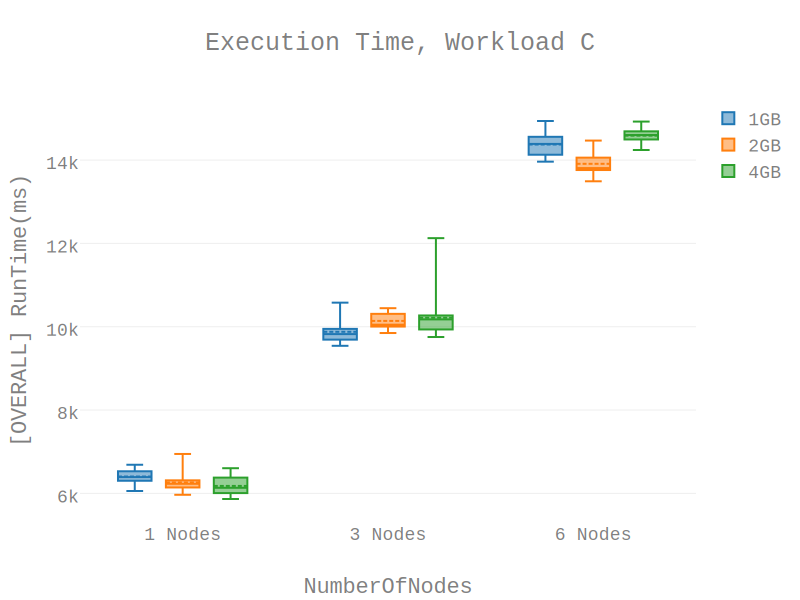
\includegraphics[width=5.5in]{Figures/figures-wlc_fig4.pdf}
\caption{}
\label{figures-wlc_fig4}
\end{figure}



\subsubsection{Ordinal Statistics}
This section will describe some of the summary statistics that describe the data.  

The summary statistics for Workload C performed on the virtual machines are in Tables \ref{table:summary_table_c_1GB_vm_nodal}, \ref{table:summary_table_c_2GB_vm_nodal}, and \ref{table:summary_table_c_4GB_vm_nodal}.
\begin{table}
\begin{tabular}{lrrrr}
\toprule
cluster\_size &     1.0 &     3.0 &     6.0 &  Overall \\
\midrule
25\%   & 6.3e+03 & 9.7e+03 & 1.4e+04 &  6.5e+03 \\
50\%   & 6.4e+03 & 9.8e+03 & 1.4e+04 &  9.8e+03 \\
75\%   & 6.5e+03 & 9.9e+03 & 1.5e+04 &  1.4e+04 \\
count &      21 &      21 &      21 &       63 \\
max   & 6.7e+03 & 1.1e+04 & 1.5e+04 &  1.5e+04 \\
mean  & 6.4e+03 & 9.9e+03 & 1.4e+04 &    1e+04 \\
min   & 6.1e+03 & 9.5e+03 & 1.4e+04 &  6.1e+03 \\
range & 6.3e+02 &   1e+03 & 9.8e+02 &  8.9e+03 \\
std   & 1.7e+02 & 2.6e+02 &   3e+02 &  3.3e+03 \\
\bottomrule
\end{tabular}
\caption{Summary Statistics for Workload C performed on a 1GB virtual machine node over a(n)nodal network.  Except for count, all values are in milliseconds.}
\label{table:summary_table_c_1GB_vm_nodal}
\end{table}

\begin{table}
\begin{tabular}{lrrrr}
\toprule
cluster\_size &     1.0 &     3.0 &     6.0 &  Overall \\
\midrule
25\%   &   6e+03 & 9.9e+03 & 1.4e+04 &  6.4e+03 \\
50\%   & 6.1e+03 &   1e+04 & 1.5e+04 &    1e+04 \\
75\%   & 6.4e+03 &   1e+04 & 1.5e+04 &  1.4e+04 \\
count &      21 &      21 &      21 &       63 \\
max   & 6.6e+03 & 1.2e+04 & 1.5e+04 &  1.5e+04 \\
mean  & 6.2e+03 &   1e+04 & 1.5e+04 &    1e+04 \\
min   & 5.9e+03 & 9.8e+03 & 1.4e+04 &  5.9e+03 \\
range & 7.4e+02 & 2.4e+03 & 6.8e+02 &  9.1e+03 \\
std   & 2.3e+02 &   5e+02 & 1.8e+02 &  3.5e+03 \\
\bottomrule
\end{tabular}
\caption{Summary Statistics for Workload C performed on a 4GB virtual machine node over a(n)nodal network.  Except for count, all values are in milliseconds.}
\label{table:summary_table_c_4GB_vm_nodal}
\end{table}




\subsubsection{Analysis}
This section will take a more in-depth look at the data.


\begin{table}[H]
\centering
\begin{tabular}{rrrrrr}
\toprule
 cluster\_size &   slope &  intercept &  r\_value &  p\_value &  std\_err \\
\midrule
            1 &     -71 &    6.4e+03 &    -0.39 &   0.0014 &       21 \\
            3 &   1e+02 &    9.8e+03 &     0.35 &   0.0046 &       35 \\
            6 & 1.1e+02 &    1.4e+04 &     0.36 &   0.0035 &       36 \\
\bottomrule
\end{tabular}
\caption{Linear Regression over amount of RAM}
\label{table:ram_v_ram_c}
\end{table}



\subsection{Implementation on Raspberry Pi}
\subsubsection{Initial Observations}
The results are displayed in Figure \ref{figures-wlc_fig10}.  \begin{figure}[h]
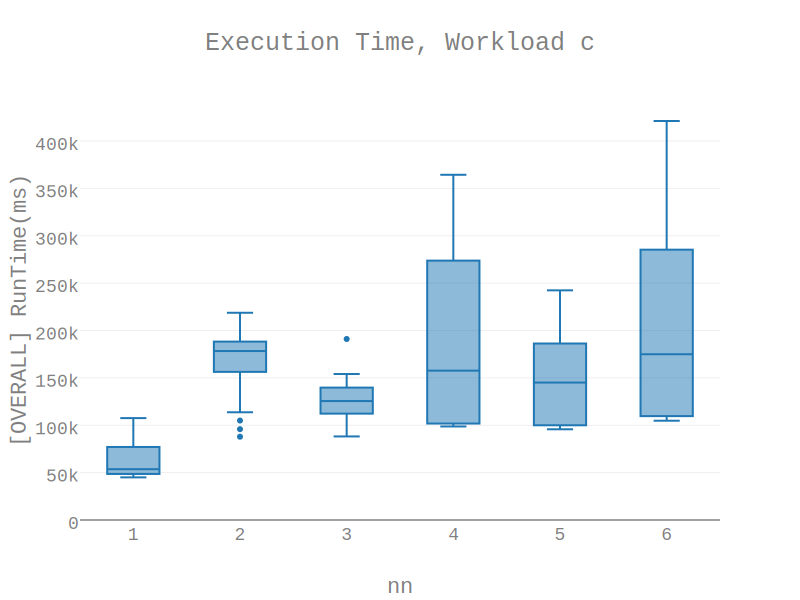
\includegraphics[width=5.5in]{Figures/figures-wlc_fig10.pdf}
\caption{}
\label{figures-wlc_fig10}
\end{figure}



\subsubsection{Ordinal Statistics}
This section will describe some of the summary statistics that describe the data.  

The summary statistics for Workload C performed on the limited hardware, Raspberry Pi, on the Ethernet local area network are in Table \ref{table:summary_table_c_1GB_rp_eth}.
\begin{table}
\begin{tabular}{lrrrrrrr}
\toprule
cluster\_size &     1.0 &     2.0 &     3.0 &     4.0 &     5.0 &     6.0 &  Overall \\
\midrule
25\%   & 4.7e+04 & 1.8e+05 & 1.1e+05 &   1e+05 & 9.7e+04 & 1.1e+05 &  9.8e+04 \\
50\%   & 4.9e+04 & 1.8e+05 & 1.1e+05 &   1e+05 & 9.8e+04 & 1.1e+05 &    1e+05 \\
75\%   &   5e+04 & 1.8e+05 & 1.1e+05 &   1e+05 &   1e+05 & 1.1e+05 &  1.1e+05 \\
count &      21 &      21 &      21 &      21 &      21 &      21 &  1.3e+02 \\
max   &   5e+04 & 1.9e+05 & 1.3e+05 &   1e+05 &   1e+05 & 1.1e+05 &  1.9e+05 \\
mean  & 4.8e+04 & 1.8e+05 & 1.1e+05 &   1e+05 & 9.9e+04 & 1.1e+05 &  1.1e+05 \\
min   & 4.5e+04 & 1.6e+05 & 1.1e+05 &   1e+05 & 9.6e+04 &   1e+05 &  4.5e+04 \\
range & 5.4e+03 & 3.2e+04 & 1.7e+04 &   4e+03 &   7e+03 & 8.1e+03 &  1.5e+05 \\
std   & 1.8e+03 & 6.7e+03 & 3.2e+03 & 1.2e+03 &   2e+03 & 2.1e+03 &  3.9e+04 \\
\bottomrule
\end{tabular}
\caption{Summary Statistics for Workload C performed on a 1GB limited hardware, Raspberry Pi node over a(n)Ethernet network.  Except for count, all values are in milliseconds.}
\label{table:summary_table_c_1GB_rp_eth}
\end{table}



\subsubsection{Analysis}
This section will take a more in-depth look at the data.


\begin{table}[H]
\centering
\begin{tabular}{rrrrr}
\toprule
  slope &  intercept &  r\_value &  p\_value &  std\_err \\
\midrule
1.4e+03 &      1e+05 &     0.06 &      0.5 &    2e+03 \\
\bottomrule
\end{tabular}
\caption{Linear Regression over Cluster Size, Workload c}
\label{table:rp_only_c}
\end{table}



\subsection{Raspberry Pi vs Reference Value}
\subsubsection{Initial Observations}
The results are displayed in Figure \ref{figures-wlc_fig6}.  The performance of the limited hardware, the Raspberry Pi, seems comparable with the results from the more appropriate in the other paper. In addition, there is no reason to suspect a significant differential in the overall pattern with respect to scalability: performance over cluster size. \begin{figure}[h]
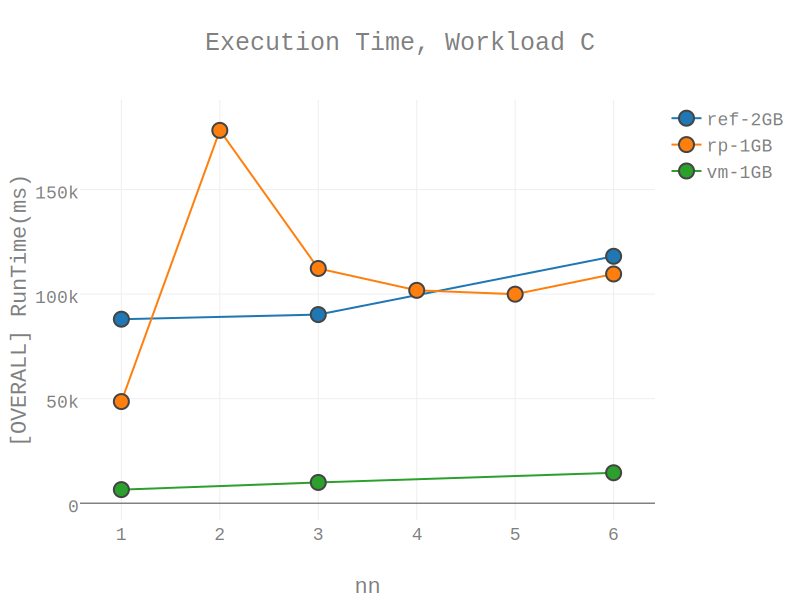
\includegraphics[width=5.5in]{Figures/figures-wlc_fig6.pdf}
\caption{}
\label{figures-wlc_fig6}
\end{figure}



\subsubsection{Ordinal Statistics}
This section will describe some of the summary statistics that describe the data.  

The summary statistics for Workload C performed on the limited hardware, Raspberry Pi, on the Ethernet local area network are in Table \ref{table:summary_table_c_1GB_rp_eth}.



\subsubsection{Analysis}
This section will take a more in-depth look at the data.
:::something went wrong generating the speedup analysis tables:::

\subsection{Raspberry Pi vs Virtual Machine}
\subsubsection{Initial Observations}
The results are displayed in Figure \ref{figures-wlc_fig6}.  As expected, there is a significant differential between the limited hardware, the Raspberry Pi configuration and the virtual machine.  However, it is not clear if this is linear across cluster size. 

\subsubsection{Ordinal Statistics}
This section will describe some of the summary statistics that describe the data.  

The summary statistics for Workload C performed on the virtual machines are in Tables \ref{table:summary_table_c_1GB_vm_nodal}, \ref{table:summary_table_c_2GB_vm_nodal}, and \ref{table:summary_table_c_4GB_vm_nodal}.
The summary statistics for Workload C performed on the limited hardware, Raspberry Pi, on the Ethernet local area network are in Table \ref{table:summary_table_c_1GB_rp_eth}.



\subsubsection{Analysis}
This section will take a more in-depth look at the data.




\begin{table}[H]
\centering
\begin{tabular}{lrrrrr}
\toprule
cluster\_size &   slope &  intercept &  r\_value &  p\_value &  std\_err \\
\midrule
           1 & 4.2e+04 &    6.4e+03 &        1 &  1.1e-50 &  3.9e+02 \\
           2 &     nan &        nan &        0 &        1 &      inf \\
           3 &   1e+05 &    9.9e+03 &        1 &  2.4e-56 &    7e+02 \\
           4 &     nan &        nan &        0 &        1 &      inf \\
           5 &     nan &        nan &        0 &        1 &      inf \\
           6 & 9.4e+04 &    1.4e+04 &        1 &  1.2e-61 &  4.7e+02 \\
     OVERALL & 9.8e+04 &      1e+04 &     0.83 &  1.6e-48 &  4.9e+03 \\
\bottomrule
\end{tabular}
\caption{Linear Regression over the effect of limited hardware, Workload C}
\label{table:rp_v_vm_c}
\end{table}





\begin{table}[H]
\centering
\begin{tabular}{llllllll}
\toprule
{} &     0 &    1 &     2 &    3 &    4 &    5 &        6 \\
\midrule
cluster\_size         &     1 &    2 &     3 &    4 &    5 &    6 &  OVERALL \\
ratio\_max\_to\_min     &  0.15 &  NaN & 0.097 &  NaN &  NaN & 0.14 &     0.33 \\
ratio\_min\_to\_max     &  0.12 &  NaN & 0.076 &  NaN &  NaN & 0.12 &    0.032 \\
ratio\_of\_the\_means   &  0.13 &  NaN & 0.087 &  NaN &  NaN & 0.13 &    0.094 \\
ratio\_of\_the\_medians &  0.13 &  NaN & 0.087 &  NaN &  NaN & 0.13 &    0.094 \\
ratio\_of\_the\_stddevs & 0.092 &  NaN & 0.079 &  NaN &  NaN & 0.14 &    0.085 \\
\bottomrule
\end{tabular}
\caption{Speedup over the effect of limited hardware, Workload C}
\label{table:rp_v_vm_c_speedup}
\end{table}





\subsection{Wireless Links Only}
\subsubsection{Initial Observations}
The results are displayed in Figure \ref{figures-wlc_fig8}.  Although there is a general trend of increased execution time over cluster size, the oscillation that occurs between odd and even node cluster sizes is hard to miss. This may be result of the collision avoidance strategy, but further experiments would be needed to determine a more specific explanation. \begin{figure}[h]
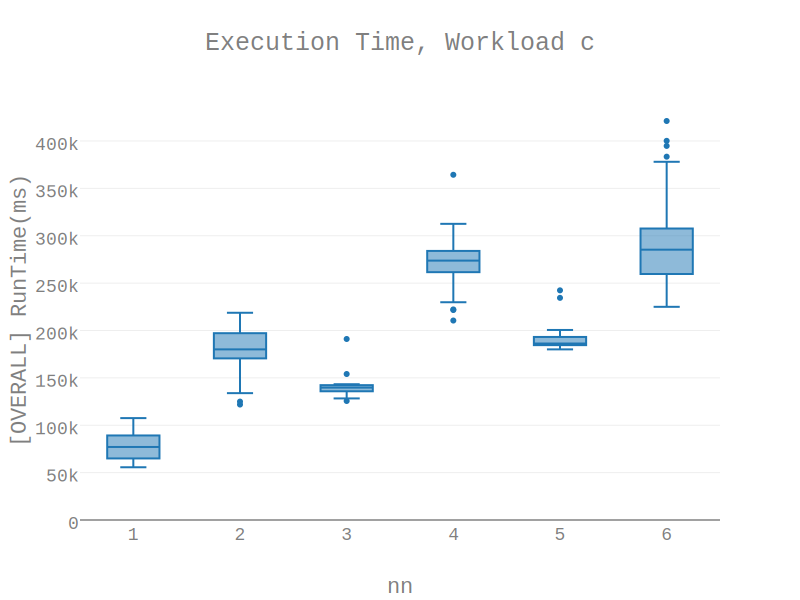
\includegraphics[width=5.5in]{Figures/figures-wlc_fig8.pdf}
\caption{}
\label{figures-wlc_fig8}
\end{figure}



\subsubsection{Ordinal Statistics}
This section will describe some of the summary statistics that describe the data.  

The summary statistics for Workload C performed on the limited hardware, Raspberry Pi, on the Ethernet local area network are in Table \ref{table:summary_table_c_1GB_rp_wlan}.
\begin{table}
\begin{tabular}{lrrrrrrr}
\toprule
cluster\_size &     1.0 &     2.0 &     3.0 &     4.0 &     5.0 &     6.0 &  Overall \\
\midrule
25\%   & 6.4e+04 & 1.8e+05 & 1.4e+05 & 2.7e+05 & 1.8e+05 & 2.5e+05 &  1.4e+05 \\
50\%   &   7e+04 & 1.9e+05 & 1.4e+05 & 2.7e+05 & 1.9e+05 & 2.7e+05 &  1.9e+05 \\
75\%   & 8.3e+04 &   2e+05 & 1.4e+05 & 2.8e+05 & 1.9e+05 & 2.9e+05 &  2.6e+05 \\
count &      21 &      21 &      21 &      21 &      21 &      21 &  1.3e+02 \\
max   & 9.4e+04 & 2.2e+05 & 1.9e+05 & 3.1e+05 & 2.4e+05 & 3.1e+05 &  3.1e+05 \\
mean  & 7.3e+04 & 1.9e+05 & 1.4e+05 & 2.8e+05 & 1.9e+05 & 2.7e+05 &  1.9e+05 \\
min   & 5.6e+04 & 1.7e+05 & 1.4e+05 & 2.3e+05 & 1.8e+05 & 2.2e+05 &  5.6e+04 \\
range & 3.8e+04 & 4.8e+04 & 5.5e+04 & 8.3e+04 & 6.2e+04 & 8.3e+04 &  2.6e+05 \\
std   & 1.2e+04 & 1.5e+04 & 1.1e+04 & 1.9e+04 & 1.6e+04 & 2.7e+04 &  7.2e+04 \\
\bottomrule
\end{tabular}
\caption{Summary Statistics for Workload C performed on a 1GB limited hardware, Raspberry Pi node over a(n)802.11a/b/g/n network.  Except for count, all values are in milliseconds.}
\label{table:summary_table_c_1GB_rp_wlan}
\end{table}



\subsubsection{Analysis}
This section will take a more in-depth look at the data.


\begin{table}[H]
\centering
\begin{tabular}{rrrrr}
\toprule
  slope &  intercept &  r\_value &  p\_value &  std\_err \\
\midrule
3.1e+04 &      8e+04 &     0.75 &  6.7e-24 &  2.5e+03 \\
\bottomrule
\end{tabular}
\caption{Linear Regression over Cluster Size, Workload c}
\label{table:wlan_only_c}
\end{table}



\subsection{Wireless Links vs Wired Links}
\subsubsection{Initial Observations}
The results are displayed in Figures \ref{figures-wlc_fig7} and \ref{figures-wlc_fig9}.  For 1, 2, and 3-node clusters, despite the expected  disparity in execution time, the wired and wireless trends seem to follow each other.  However, from 3 nodes up through 6 nodes, the execution times starts to diverge, suggesting that the wireless has a increasing effect as the number of nodes increases. \begin{figure}[h]
\includegraphics[width=5.5in]{Figures/figures-wlc_fig7.pdf}
\caption{}
\label{figures-wlc_fig7}
\end{figure}

\begin{figure}[h]
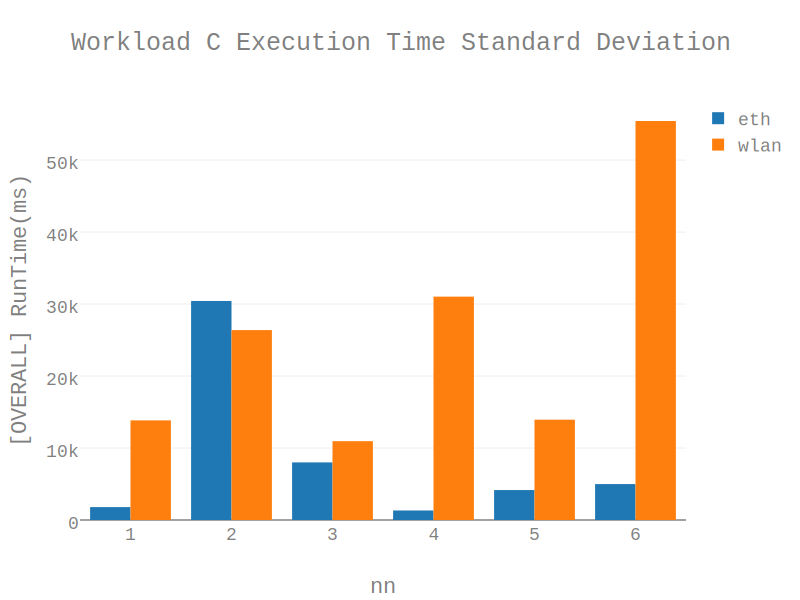
\includegraphics[width=5.5in]{Figures/figures-wlc_fig9.pdf}
\caption{}
\label{figures-wlc_fig9}
\end{figure}



\subsubsection{Ordinal Statistics}
This section will describe some of the summary statistics that describe the data.  

The summary statistics for Workload C performed on the limited hardware, Raspberry Pi, on the Ethernet local area network are in Table \ref{table:summary_table_c_1GB_rp_eth}.
The summary statistics for Workload C performed on the limited hardware, Raspberry Pi, on the Ethernet local area network are in Table \ref{table:summary_table_c_1GB_rp_wlan}.



\subsubsection{Analysis}
This section will take a more in-depth look at the data.




\begin{table}[H]
\centering
\begin{tabular}{lrrrrr}
\toprule
cluster\_size &   slope &  intercept &  r\_value &  p\_value &  std\_err \\
\midrule
           1 & 2.5e+04 &    4.8e+04 &     0.83 &  1.3e-11 &  2.6e+03 \\
           2 & 1.1e+04 &    1.8e+05 &     0.43 &   0.0049 &  3.7e+03 \\
           3 &   3e+04 &    1.1e+05 &     0.88 &  2.2e-14 &  2.6e+03 \\
           4 & 1.7e+05 &      1e+05 &     0.99 &  2.5e-34 &  4.2e+03 \\
           5 & 9.2e+04 &    9.9e+04 &     0.97 &  2.7e-26 &  3.6e+03 \\
           6 & 1.6e+05 &    1.1e+05 &     0.97 &  7.4e-27 &    6e+03 \\
     OVERALL & 8.1e+04 &    1.1e+05 &     0.58 &    9e-24 &  7.3e+03 \\
\bottomrule
\end{tabular}
\caption{Linear Regression over the effect of 802.11 links, Workload C}
\label{table:wlan_v_eth_c}
\end{table}





\begin{table}[H]
\centering
\begin{tabular}{llllllll}
\toprule
{} &    0 &    1 &    2 &     3 &    4 &     5 &        6 \\
\midrule
cluster\_size         &    1 &    2 &    3 &     4 &    5 &     6 &  OVERALL \\
ratio\_max\_to\_min     & 0.91 &  1.1 & 0.92 &  0.46 & 0.57 &   0.5 &      3.4 \\
ratio\_min\_to\_max     & 0.48 & 0.73 & 0.57 &  0.32 &  0.4 &  0.34 &     0.14 \\
ratio\_of\_the\_means   & 0.66 & 0.94 & 0.79 &  0.37 & 0.52 &  0.41 &     0.57 \\
ratio\_of\_the\_medians & 0.69 & 0.94 &  0.8 &  0.38 & 0.53 &   0.4 &     0.56 \\
ratio\_of\_the\_stddevs & 0.15 & 0.43 & 0.28 & 0.061 & 0.12 & 0.078 &     0.54 \\
\bottomrule
\end{tabular}
\caption{Speedup over the effect of 802.11 links, Workload C}
\label{table:wlan_v_eth_c_speedup}
\end{table}





\section{Results for Workload E}
\subsection{Comparing Existing Work: Virtual Machine vs the Reference Value}
\subsubsection{Initial Observations}
The result medians are displayed in Figure \ref{figures-wle_fig5}.  As expected, the virtual machine results imply much, much less execution time compared to the reference value, presumably accounting for diminished network latency. For the reference value, it seems a higher cluster size seems to imply a cost, but a cost that decreases as the cluster size increases. However,  further analysis would be required to see if this is not just the product of normal variation.  Because of the high contrast, it difficult to reach any initial predictions for virtual machine.  The flat curve may just be an illusion, a minimization of the differences due to the scale of the graph.  \begin{figure}[h]
\includegraphics[width=5.5in]{Figures/figures-wle_fig1.pdf}
\caption{}
\label{figures-wle_fig1}
\end{figure}

\begin{figure}[h]
\includegraphics[width=5.5in]{Figures/figures-wle_fig5.pdf}
\caption{}
\label{figures-wle_fig5}
\end{figure}



\subsubsection{Ordinal Statistics}
This section will describe some of the summary statistics that describe the data.  

The summary statistics for Workload E performed on the virtual machines are in Tables \ref{table:summary_table_e_1GB_vm_nodal}, \ref{table:summary_table_e_2GB_vm_nodal}, and \ref{table:summary_table_e_4GB_vm_nodal}.
\begin{table}
\begin{tabular}{lrrrr}
\toprule
cluster\_size &     1.0 &     3.0 &     6.0 &  Overall \\
\midrule
25\%   & 2.3e+04 & 2.4e+04 & 3.1e+04 &  2.4e+04 \\
50\%   & 2.5e+04 & 2.4e+04 & 3.1e+04 &  2.6e+04 \\
75\%   & 2.6e+04 & 2.5e+04 & 3.2e+04 &  3.1e+04 \\
count &      21 &      21 &      21 &       63 \\
max   & 2.9e+04 & 2.6e+04 & 3.3e+04 &  3.3e+04 \\
mean  & 2.5e+04 & 2.5e+04 & 3.1e+04 &  2.7e+04 \\
min   & 2.1e+04 & 2.3e+04 & 3.1e+04 &  2.1e+04 \\
range &   8e+03 &   3e+03 &   2e+03 &  1.1e+04 \\
std   & 2.2e+03 & 7.5e+02 & 5.3e+02 &  3.5e+03 \\
\bottomrule
\end{tabular}
\caption{Summary Statistics for Workload E performed on a 2GB virtual machine node over a(n)nodal network.  Except for count, all values are in milliseconds.}
\label{table:summary_table_e_2GB_vm_nodal}
\end{table}



\subsubsection{Analysis}
This section will take a more in-depth look at the data.
:::something went wrong generating the speedup analysis tables:::

\subsection{1GB RAM vs 2GB RAM vs 4GB RAM}
\subsubsection{Initial Observations}
The results are displayed in Figure \ref{figures-wle_fig4}.  First of all, the performance for the a one-node cluster differs significantly between 1GB RAM andall other cases.  While this could be some kind of implementation error, it is best not to draw any conclusions fromthis. It would be best to run these tests again, possibly switching the order to eliminate the possible effect of interference or a mix-up of data. That one case aside, the amount of RAM seems to have had an effect on the results, but there doesnot seem to be any predictive relationship that holds true across cluster sizes. \begin{figure}[h]
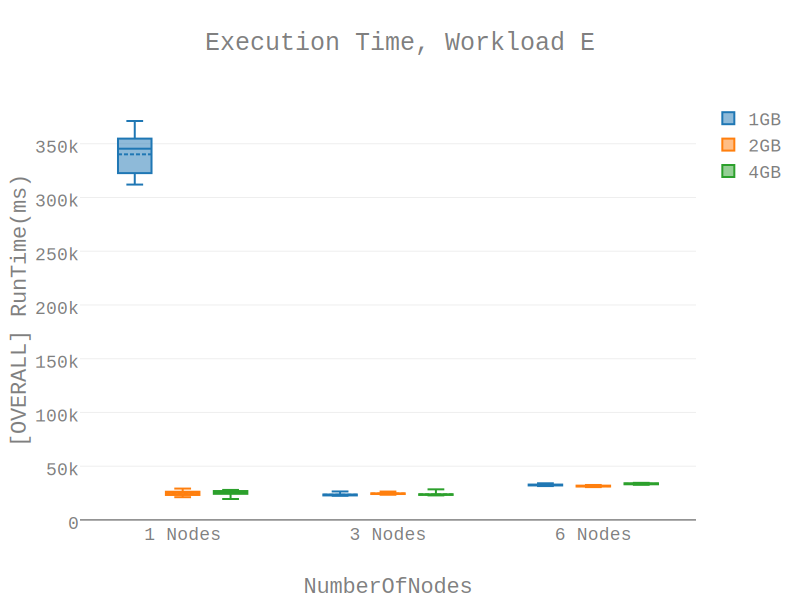
\includegraphics[width=5.5in]{Figures/figures-wle_fig4.pdf}
\caption{}
\label{figures-wle_fig4}
\end{figure}



\subsubsection{Ordinal Statistics}
This section will describe some of the summary statistics that describe the data.  

The summary statistics for Workload E performed on the virtual machines are in Tables \ref{table:summary_table_e_1GB_vm_nodal}, \ref{table:summary_table_e_2GB_vm_nodal}, and \ref{table:summary_table_e_4GB_vm_nodal}.
\begin{table}
\begin{tabular}{lrrrr}
\toprule
cluster\_size &     1.0 &     3.0 &     6.0 &  Overall \\
\midrule
25\%   & 3.2e+05 & 2.3e+04 & 3.2e+04 &    3e+04 \\
50\%   & 3.5e+05 & 2.3e+04 & 3.2e+04 &  1.7e+05 \\
75\%   & 3.5e+05 & 2.4e+04 & 3.3e+04 &  3.4e+05 \\
count &      42 &      21 &      21 &       84 \\
max   & 3.7e+05 & 2.6e+04 & 3.4e+04 &  3.7e+05 \\
mean  & 3.4e+05 & 2.3e+04 & 3.2e+04 &  1.8e+05 \\
min   & 3.1e+05 & 2.2e+04 & 3.2e+04 &  2.2e+04 \\
range & 5.9e+04 & 4.1e+03 & 2.6e+03 &  3.5e+05 \\
std   & 1.8e+04 &   1e+03 & 6.1e+02 &  1.6e+05 \\
\bottomrule
\end{tabular}
\caption{Summary Statistics for Workload E performed on a 1GB virtual machine node over a(n)nodal network.  Except for count, all values are in milliseconds.}
\label{table:summary_table_e_1GB_vm_nodal}
\end{table}

\begin{table}
\begin{tabular}{lrrrr}
\toprule
cluster\_size &     1.0 &     3.0 &     6.0 &  Overall \\
\midrule
25\%   & 2.4e+04 & 2.3e+04 & 3.3e+04 &  2.4e+04 \\
50\%   & 2.5e+04 & 2.4e+04 & 3.4e+04 &  2.5e+04 \\
75\%   & 2.7e+04 & 2.4e+04 & 3.4e+04 &  3.3e+04 \\
count &      21 &      21 &      21 &       63 \\
max   & 2.8e+04 & 2.8e+04 & 3.5e+04 &  3.5e+04 \\
mean  & 2.5e+04 & 2.4e+04 & 3.4e+04 &  2.8e+04 \\
min   & 1.9e+04 & 2.3e+04 & 3.3e+04 &  1.9e+04 \\
range & 8.4e+03 & 5.6e+03 & 1.9e+03 &  1.5e+04 \\
std   & 2.1e+03 & 1.2e+03 & 6.1e+02 &  4.6e+03 \\
\bottomrule
\end{tabular}
\caption{Summary Statistics for Workload E performed on a 4GB virtual machine node over a(n)nodal network.  Except for count, all values are in milliseconds.}
\label{table:summary_table_e_4GB_vm_nodal}
\end{table}




\subsubsection{Analysis}
This section will take a more in-depth look at the data.


\begin{table}[H]
\centering
\begin{tabular}{rrrrrr}
\toprule
 cluster\_size &    slope &  intercept &  r\_value &  p\_value &  std\_err \\
\midrule
            1 & -1.1e+05 &    3.9e+05 &    -0.81 &    5e-21 &  8.3e+03 \\
            3 &       32 &    2.4e+04 &    0.037 &     0.77 &  1.1e+02 \\
            6 &  4.7e+02 &    3.1e+04 &     0.57 &  1.4e-06 &       88 \\
\bottomrule
\end{tabular}
\caption{Linear Regression over amount of RAM}
\label{table:ram_v_ram_e}
\end{table}



\subsection{Implementation on Raspberry Pi}
\subsubsection{Initial Observations}
The results are displayed in Figure \ref{figures-wle_fig10}.  \begin{figure}[h]
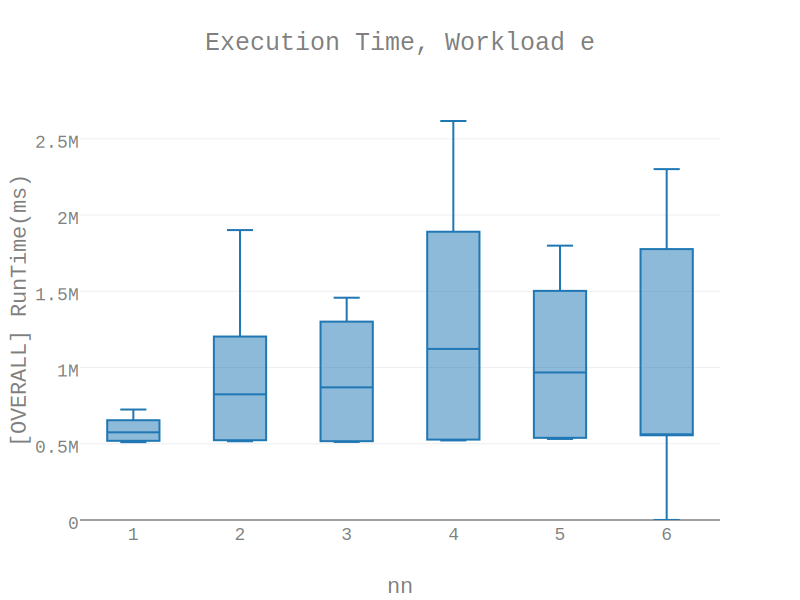
\includegraphics[width=5.5in]{Figures/figures-wle_fig10.pdf}
\caption{}
\label{figures-wle_fig10}
\end{figure}



\subsubsection{Ordinal Statistics}
This section will describe some of the summary statistics that describe the data.  

The summary statistics for Workload E performed on the limited hardware, Raspberry Pi, on the Ethernet local area network are in Table \ref{table:summary_table_e_1GB_rp_eth}.
\begin{table}
\begin{tabular}{lrrrrrrr}
\toprule
cluster\_size &     1.0 &     2.0 &     3.0 &     4.0 &     5.0 &     6.0 &  Overall \\
\midrule
25\%   & 5.2e+05 & 5.2e+05 & 5.1e+05 & 5.3e+05 & 5.4e+05 & 5.6e+05 &  5.2e+05 \\
50\%   & 5.2e+05 & 5.2e+05 & 5.2e+05 & 5.3e+05 & 5.4e+05 & 5.6e+05 &  5.3e+05 \\
75\%   & 5.2e+05 & 5.3e+05 & 5.2e+05 & 5.4e+05 & 5.4e+05 & 5.6e+05 &  5.4e+05 \\
count &      21 &      21 &      21 &      21 &      21 &      21 &  1.3e+02 \\
max   & 5.2e+05 & 5.3e+05 & 5.3e+05 & 5.4e+05 & 5.4e+05 & 5.7e+05 &  5.7e+05 \\
mean  & 5.2e+05 & 5.2e+05 & 5.2e+05 & 5.3e+05 & 5.4e+05 & 5.6e+05 &  5.3e+05 \\
min   & 5.2e+05 & 5.2e+05 & 5.1e+05 & 5.2e+05 & 5.3e+05 & 5.6e+05 &  5.1e+05 \\
range & 8.3e+03 & 1.3e+04 &   2e+04 & 1.8e+04 & 9.9e+03 &   1e+04 &  5.3e+04 \\
std   & 2.1e+03 & 3.5e+03 & 5.5e+03 &   6e+03 & 2.8e+03 &   3e+03 &  1.5e+04 \\
\bottomrule
\end{tabular}
\caption{Summary Statistics for Workload E performed on a 1GB limited hardware, Raspberry Pi node over a(n)Ethernet network.  Except for count, all values are in milliseconds.}
\label{table:summary_table_e_1GB_rp_eth}
\end{table}



\subsubsection{Analysis}
This section will take a more in-depth look at the data.


\begin{table}[H]
\centering
\begin{tabular}{rrrrr}
\toprule
  slope &  intercept &  r\_value &  p\_value &  std\_err \\
\midrule
7.2e+03 &    5.1e+05 &     0.84 &  2.8e-35 &  4.1e+02 \\
\bottomrule
\end{tabular}
\caption{Linear Regression over Cluster Size, Workload e}
\label{table:rp_only_e}
\end{table}



\subsection{Raspberry Pi vs Reference Value}
\subsubsection{Initial Observations}
The results are displayed in Figure \ref{figures-wle_fig6}.  These medians seem to indicate, that for this workload, any effect of the Raspberry Pi is exacerbated with this particular workload. \begin{figure}[h]
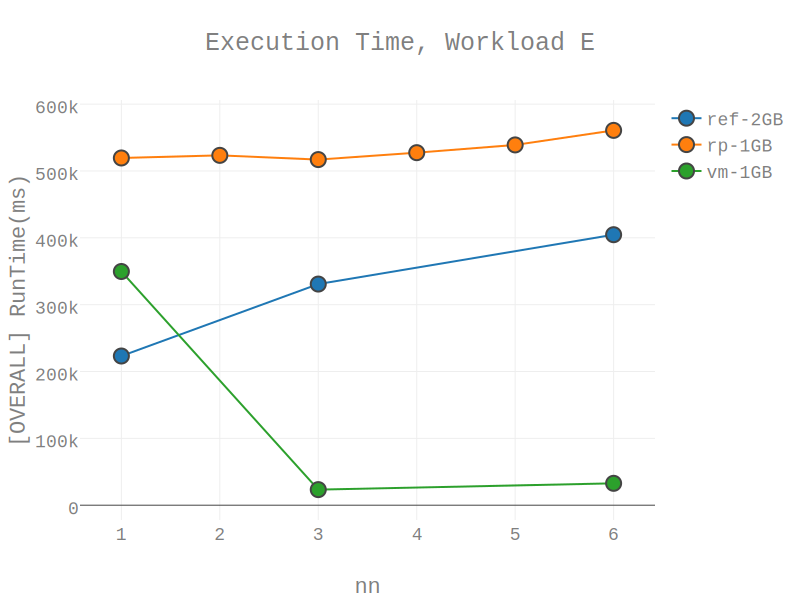
\includegraphics[width=5.5in]{Figures/figures-wle_fig6.pdf}
\caption{}
\label{figures-wle_fig6}
\end{figure}



\subsubsection{Ordinal Statistics}
This section will describe some of the summary statistics that describe the data.  

The summary statistics for Workload E performed on the limited hardware, Raspberry Pi, on the Ethernet local area network are in Table \ref{table:summary_table_e_1GB_rp_eth}.



\subsubsection{Analysis}
This section will take a more in-depth look at the data.
:::something went wrong generating the speedup analysis tables:::

\subsection{Raspberry Pi vs Virtual Machine}
\subsubsection{Initial Observations}
The results are displayed in Figure \ref{figures-wle_fig6}.  As expected, there is a significant differential between the limited hardware, the Raspberry Pi configuration and the virtual machine.  However, it is not clear if this is linear across cluster size. 

\subsubsection{Ordinal Statistics}
This section will describe some of the summary statistics that describe the data.  

The summary statistics for Workload E performed on the virtual machines are in Tables \ref{table:summary_table_e_1GB_vm_nodal}, \ref{table:summary_table_e_2GB_vm_nodal}, and \ref{table:summary_table_e_4GB_vm_nodal}.
The summary statistics for Workload E performed on the limited hardware, Raspberry Pi, on the Ethernet local area network are in Table \ref{table:summary_table_e_1GB_rp_eth}.



\subsubsection{Analysis}
This section will take a more in-depth look at the data.




\begin{table}[H]
\centering
\begin{tabular}{lrrrrr}
\toprule
cluster\_size &   slope &  intercept &  r\_value &  p\_value &  std\_err \\
\midrule
           1 & 1.8e+05 &    3.4e+05 &     0.99 &    2e-49 &  3.9e+03 \\
           2 &     nan &        nan &        0 &        1 &      inf \\
           3 &   5e+05 &    2.3e+04 &        1 &  8.9e-74 &  1.2e+03 \\
           4 &     nan &        nan &        0 &        1 &      inf \\
           5 &     nan &        nan &        0 &        1 &      inf \\
           6 & 5.3e+05 &    3.2e+04 &        1 &  1.3e-85 &  6.6e+02 \\
     OVERALL & 3.5e+05 &    1.8e+05 &     0.86 &  1.3e-63 &  1.4e+04 \\
\bottomrule
\end{tabular}
\caption{Linear Regression over the effect of limited hardware, Workload E}
\label{table:rp_v_vm_e}
\end{table}





\begin{table}[H]
\centering
\begin{tabular}{llllllll}
\toprule
{} &    0 &    1 &     2 &    3 &    4 &     5 &        6 \\
\midrule
cluster\_size         &    1 &    2 &     3 &    4 &    5 &     6 &  OVERALL \\
ratio\_max\_to\_min     & 0.72 &  NaN & 0.052 &  NaN &  NaN & 0.061 &     0.72 \\
ratio\_min\_to\_max     &  0.6 &  NaN & 0.042 &  NaN &  NaN & 0.056 &     0.04 \\
ratio\_of\_the\_means   & 0.65 &  NaN & 0.045 &  NaN &  NaN & 0.058 &     0.35 \\
ratio\_of\_the\_medians & 0.66 &  NaN & 0.045 &  NaN &  NaN & 0.058 &     0.33 \\
ratio\_of\_the\_stddevs &  8.4 &  NaN &  0.18 &  NaN &  NaN &  0.21 &       11 \\
\bottomrule
\end{tabular}
\caption{Speedup over the effect of limited hardware, Workload E}
\label{table:rp_v_vm_e_speedup}
\end{table}





\subsection{Wireless Links Only}
\subsubsection{Initial Observations}
The results are displayed in Figure \ref{figures-wle_fig8}.  Although there is a general trend of increased execution time over cluster size, the oscillation that occurs between odd and even node cluster sizes is hard to miss. This may be result of the collision avoidance strategy, but further experiments would be needed to determine a more specific explanation. \begin{figure}[h]
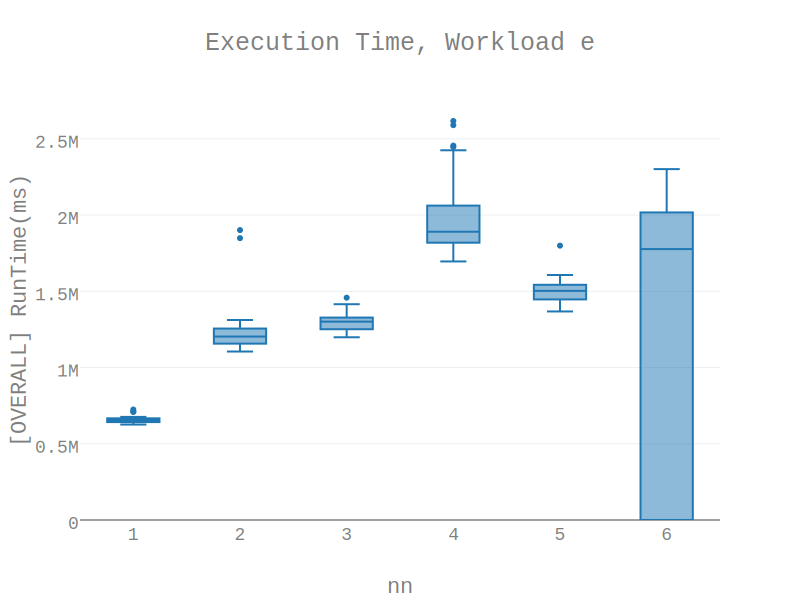
\includegraphics[width=5.5in]{Figures/figures-wle_fig8.pdf}
\caption{}
\label{figures-wle_fig8}
\end{figure}



\subsubsection{Ordinal Statistics}
This section will describe some of the summary statistics that describe the data.  

The summary statistics for Workload E performed on the limited hardware, Raspberry Pi, on the Ethernet local area network are in Table \ref{table:summary_table_e_1GB_rp_wlan}.
\begin{table}
\begin{tabular}{lrrrrrrr}
\toprule
cluster\_size &     1.0 &     2.0 &     3.0 &     4.0 &     5.0 &     6.0 &  Overall \\
\midrule
25\%   & 6.4e+05 & 1.2e+06 & 1.3e+06 & 1.8e+06 & 1.4e+06 & 2.6e+02 &  6.8e+05 \\
50\%   & 6.5e+05 & 1.2e+06 & 1.3e+06 & 1.8e+06 & 1.5e+06 & 2.8e+02 &  1.3e+06 \\
75\%   & 6.6e+05 & 1.3e+06 & 1.3e+06 & 1.9e+06 & 1.5e+06 & 1.8e+06 &  1.6e+06 \\
count &      21 &      21 &      21 &      21 &      21 &      21 &  1.3e+02 \\
max   & 7.2e+05 & 1.9e+06 & 1.5e+06 & 2.5e+06 & 1.6e+06 &   2e+06 &  2.5e+06 \\
mean  & 6.5e+05 & 1.3e+06 & 1.3e+06 & 1.9e+06 & 1.5e+06 & 6.9e+05 &  1.2e+06 \\
min   & 6.3e+05 & 1.1e+06 & 1.2e+06 & 1.7e+06 & 1.4e+06 & 2.6e+02 &  2.6e+02 \\
range & 9.9e+04 &   8e+05 & 2.6e+05 & 7.6e+05 & 2.4e+05 &   2e+06 &  2.5e+06 \\
std   & 2.4e+04 & 2.1e+05 & 6.4e+04 & 1.7e+05 & 6.8e+04 &   9e+05 &  5.8e+05 \\
\bottomrule
\end{tabular}
\caption{Summary Statistics for Workload E performed on a 1GB limited hardware, Raspberry Pi node over a(n)802.11a/b/g/n network.  Except for count, all values are in milliseconds.}
\label{table:summary_table_e_1GB_rp_wlan}
\end{table}



\subsubsection{Analysis}
This section will take a more in-depth look at the data.


\begin{table}[H]
\centering
\begin{tabular}{rrrrr}
\toprule
  slope &  intercept &  r\_value &  p\_value &  std\_err \\
\midrule
4.1e+04 &    1.1e+06 &     0.12 &     0.18 &    3e+04 \\
\bottomrule
\end{tabular}
\caption{Linear Regression over Cluster Size, Workload e}
\label{table:wlan_only_e}
\end{table}



\subsection{Wireless Links vs Wired Links}
\subsubsection{Initial Observations}
The results are displayed in Figures \ref{figures-wle_fig7} and \ref{figures-wle_fig9}.  For 1, 2, and 3-node clusters, despite the expected  disparity in execution time, the wired and wireless trends seem to follow each other.  However, from 3 nodes up through 6 nodes, the execution times starts to diverge, suggesting that the wireless has a increasing effect as the number of nodes increases. \begin{figure}[h]
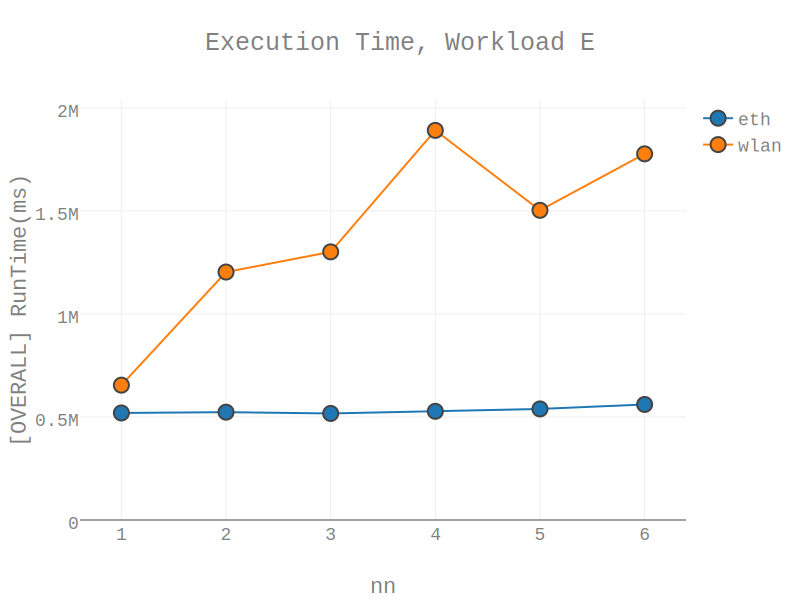
\includegraphics[width=5.5in]{Figures/figures-wle_fig7.pdf}
\caption{}
\label{figures-wle_fig7}
\end{figure}

\begin{figure}[h]
\includegraphics[width=5.5in]{Figures/figures-wle_fig9.pdf}
\caption{}
\label{figures-wle_fig9}
\end{figure}



\subsubsection{Ordinal Statistics}
This section will describe some of the summary statistics that describe the data.  

The summary statistics for Workload E performed on the limited hardware, Raspberry Pi, on the Ethernet local area network are in Table \ref{table:summary_table_e_1GB_rp_eth}.
The summary statistics for Workload E performed on the limited hardware, Raspberry Pi, on the Ethernet local area network are in Table \ref{table:summary_table_e_1GB_rp_wlan}.



\subsubsection{Analysis}
This section will take a more in-depth look at the data.




\begin{table}[H]
\centering
\begin{tabular}{lrrrrr}
\toprule
cluster\_size &   slope &  intercept &  r\_value &  p\_value &  std\_err \\
\midrule
           1 & 1.3e+05 &    5.2e+05 &     0.97 &    5e-26 &  5.4e+03 \\
           2 & 7.5e+05 &    5.2e+05 &     0.93 &  1.8e-19 &  4.5e+04 \\
           3 & 7.8e+05 &    5.2e+05 &     0.99 &  1.5e-39 &  1.4e+04 \\
           4 & 1.4e+06 &    5.3e+05 &     0.98 &  5.8e-32 &  3.8e+04 \\
           5 & 9.5e+05 &    5.4e+05 &        1 &  5.2e-42 &  1.5e+04 \\
           6 & 1.3e+05 &    5.6e+05 &      0.1 &     0.51 &    2e+05 \\
     OVERALL & 6.8e+05 &    5.3e+05 &     0.64 &    9e-31 &  5.2e+04 \\
\bottomrule
\end{tabular}
\caption{Linear Regression over the effect of 802.11 links, Workload E}
\label{table:wlan_v_eth_e}
\end{table}





\begin{table}[H]
\centering
\begin{tabular}{llllllll}
\toprule
{} &     0 &     1 &     2 &     3 &     4 &       5 &        6 \\
\midrule
cluster\_size         &     1 &     2 &     3 &     4 &     5 &       6 &  OVERALL \\
ratio\_max\_to\_min     &  0.84 &  0.48 &  0.44 &  0.32 &   0.4 & 2.2e+03 &  2.2e+03 \\
ratio\_min\_to\_max     &  0.71 &  0.27 &  0.35 &  0.21 &  0.33 &    0.27 &     0.21 \\
ratio\_of\_the\_means   &   0.8 &  0.41 &   0.4 &  0.28 &  0.36 &    0.81 &     0.44 \\
ratio\_of\_the\_medians &   0.8 &  0.43 &   0.4 &  0.29 &  0.36 &   2e+03 &      0.4 \\
ratio\_of\_the\_stddevs & 0.085 & 0.017 & 0.087 & 0.034 & 0.041 &  0.0033 &    0.025 \\
\bottomrule
\end{tabular}
\caption{Speedup over the effect of 802.11 links, Workload E}
\label{table:wlan_v_eth_e_speedup}
\end{table}





\section{Results for Workload I}
\subsection{1GB RAM vs 2GB RAM vs 4GB RAM}
\subsubsection{Initial Observations}
The results are displayed in Figure \ref{figures-wli_fig4}. Here there is a visible trend of 4GB RAM implying better performance results than both 1GB RAM and 2GB RAM.  However, the relationship between 1GB RAM and 2GB RAM does not seem to be predictable across cluster node sizes. \begin{figure}[h]
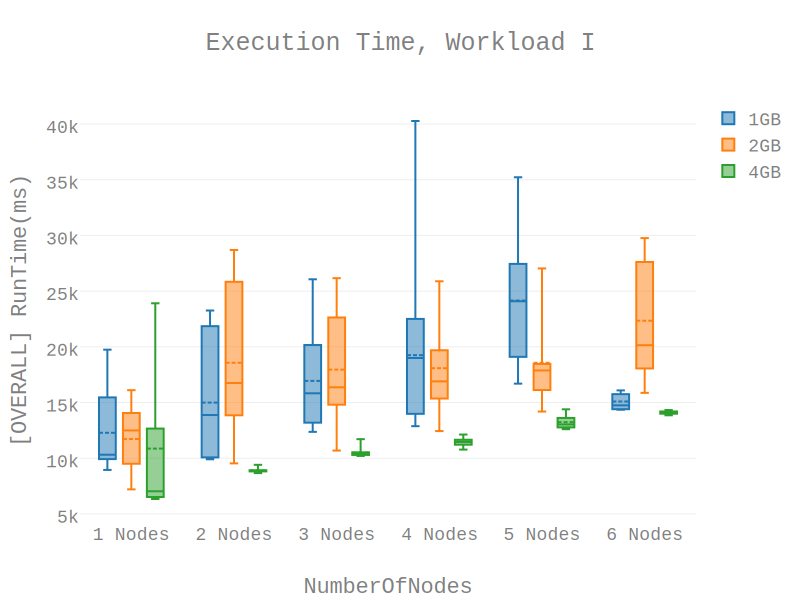
\includegraphics[width=5.5in]{Figures/figures-wli_fig4.pdf}
\caption{}
\label{figures-wli_fig4}
\end{figure}



\subsubsection{Ordinal Statistics}
This section will describe some of the summary statistics that describe the data.  

The summary statistics for Workload I performed on the virtual machines are in Tables \ref{table:summary_table_i_1GB_vm_nodal}, \ref{table:summary_table_i_2GB_vm_nodal}, and \ref{table:summary_table_i_4GB_vm_nodal}.
\begin{table}
\begin{tabular}{lrrrrrrr}
\toprule
cluster\_size &     1.0 &     2.0 &     3.0 &     4.0 &     5.0 &     6.0 &  Overall \\
\midrule
25\%   & 9.9e+03 &   1e+04 & 1.3e+04 & 1.4e+04 & 1.9e+04 & 1.4e+04 &  1.3e+04 \\
50\%   &   1e+04 & 1.4e+04 & 1.6e+04 & 1.9e+04 & 2.4e+04 & 1.5e+04 &  1.6e+04 \\
75\%   & 1.5e+04 & 2.2e+04 &   2e+04 & 2.2e+04 & 2.7e+04 & 1.6e+04 &    2e+04 \\
count &      21 &      21 &      21 &      21 &      21 &      21 &  1.3e+02 \\
max   &   2e+04 & 2.3e+04 & 2.6e+04 &   4e+04 & 3.5e+04 & 1.6e+04 &    4e+04 \\
mean  & 1.2e+04 & 1.5e+04 & 1.7e+04 & 1.9e+04 & 2.4e+04 & 1.5e+04 &  1.7e+04 \\
min   & 8.9e+03 & 9.9e+03 & 1.2e+04 & 1.3e+04 & 1.7e+04 & 1.4e+04 &  8.9e+03 \\
range & 1.1e+04 & 1.3e+04 & 1.4e+04 & 2.7e+04 & 1.9e+04 & 1.7e+03 &  3.1e+04 \\
std   & 3.7e+03 & 5.3e+03 & 4.4e+03 & 6.3e+03 & 5.7e+03 & 6.8e+02 &    6e+03 \\
\bottomrule
\end{tabular}
\caption{Summary Statistics for Workload I performed on a 1GB virtual machine node over a(n)nodal network.  Except for count, all values are in milliseconds.}
\label{table:summary_table_i_1GB_vm_nodal}
\end{table}

\begin{table}
\begin{tabular}{lrrrrrrr}
\toprule
cluster\_size &     1.0 &     2.0 &     3.0 &     4.0 &     5.0 &     6.0 &  Overall \\
\midrule
25\%   & 6.5e+03 & 8.8e+03 &   1e+04 & 1.1e+04 & 1.3e+04 & 1.4e+04 &  9.6e+03 \\
50\%   &   7e+03 & 8.9e+03 &   1e+04 & 1.1e+04 & 1.3e+04 & 1.4e+04 &  1.1e+04 \\
75\%   & 1.3e+04 & 8.9e+03 & 1.1e+04 & 1.2e+04 & 1.4e+04 & 1.4e+04 &  1.4e+04 \\
count &      21 &      21 &      21 &      21 &      21 &      21 &  1.3e+02 \\
max   & 2.4e+04 & 9.4e+03 & 1.2e+04 & 1.2e+04 & 1.4e+04 & 1.4e+04 &  2.4e+04 \\
mean  & 1.1e+04 & 8.9e+03 &   1e+04 & 1.1e+04 & 1.3e+04 & 1.4e+04 &  1.2e+04 \\
min   & 6.3e+03 & 8.7e+03 &   1e+04 & 1.1e+04 & 1.3e+04 & 1.4e+04 &  6.3e+03 \\
range & 1.8e+04 & 7.4e+02 & 1.5e+03 & 1.4e+03 & 1.8e+03 & 4.7e+02 &  1.8e+04 \\
std   & 5.7e+03 & 1.5e+02 & 3.6e+02 & 3.6e+02 & 5.5e+02 & 1.4e+02 &  2.9e+03 \\
\bottomrule
\end{tabular}
\caption{Summary Statistics for Workload I performed on a 4GB virtual machine node over a(n)nodal network.  Except for count, all values are in milliseconds.}
\label{table:summary_table_i_4GB_vm_nodal}
\end{table}




\subsubsection{Analysis}
This section will take a more in-depth look at the data.


\begin{table}[H]
\centering
\begin{tabular}{rrrrrr}
\toprule
 cluster\_size &    slope &  intercept &  r\_value &  p\_value &  std\_err \\
\midrule
            1 & -4.7e+02 &    1.3e+04 &    -0.14 &     0.28 &  4.2e+02 \\
            2 & -2.4e+03 &      2e+04 &    -0.49 &    4e-05 &  5.5e+02 \\
            3 & -2.4e+03 &    2.1e+04 &     -0.6 &  2.2e-07 &  4.1e+02 \\
            4 & -2.7e+03 &    2.3e+04 &    -0.62 &  6.7e-08 &  4.4e+02 \\
            5 & -3.5e+03 &    2.7e+04 &    -0.74 &  6.3e-12 &  4.1e+02 \\
            6 & -8.8e+02 &    1.9e+04 &    -0.24 &    0.062 &  4.6e+02 \\
\bottomrule
\end{tabular}
\caption{Linear Regression over amount of RAM}
\label{table:ram_v_ram_i}
\end{table}



\subsection{Implementation on Raspberry Pi}
\subsubsection{Initial Observations}
The results are displayed in Figure \ref{figures-wli_fig10}.  \begin{figure}[h]
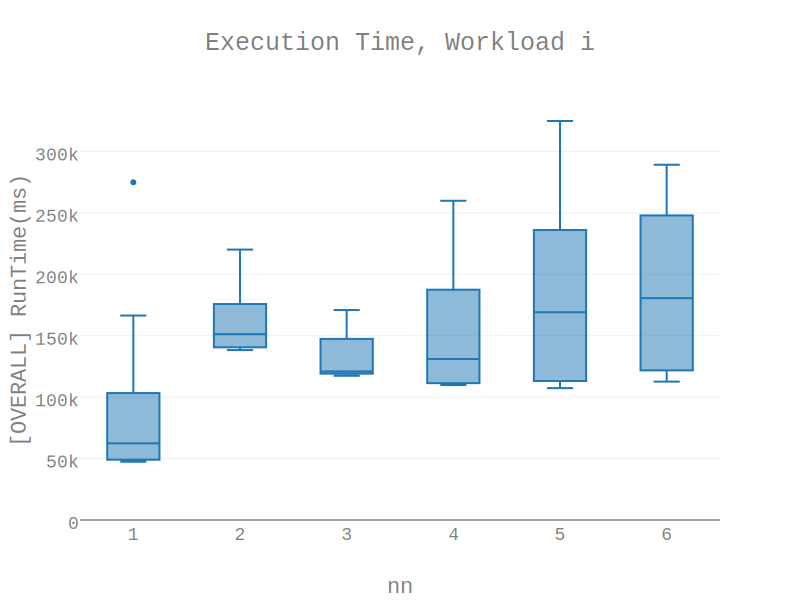
\includegraphics[width=5.5in]{Figures/figures-wli_fig10.pdf}
\caption{}
\label{figures-wli_fig10}
\end{figure}



\subsubsection{Ordinal Statistics}
This section will describe some of the summary statistics that describe the data.  

The summary statistics for Workload I performed on the limited hardware, Raspberry Pi, on the Ethernet local area network are in Table \ref{table:summary_table_i_1GB_rp_eth}.
\begin{table}
\begin{tabular}{lrrrrrrr}
\toprule
cluster\_size &     1.0 &     2.0 &     3.0 &     4.0 &     5.0 &     6.0 &  Overall \\
\midrule
25\%   & 4.9e+04 & 1.4e+05 & 1.2e+05 & 1.1e+05 & 1.1e+05 & 1.2e+05 &  1.1e+05 \\
50\%   & 4.9e+04 & 1.4e+05 & 1.2e+05 & 1.1e+05 & 1.1e+05 & 1.2e+05 &  1.2e+05 \\
75\%   &   5e+04 & 1.4e+05 & 1.2e+05 & 1.1e+05 & 1.2e+05 & 1.2e+05 &  1.2e+05 \\
count &      21 &      21 &      21 &      21 &      21 &      21 &  1.3e+02 \\
max   & 5.2e+04 & 1.4e+05 & 1.2e+05 & 1.1e+05 & 1.2e+05 & 1.3e+05 &  1.4e+05 \\
mean  & 4.9e+04 & 1.4e+05 & 1.2e+05 & 1.1e+05 & 1.1e+05 & 1.2e+05 &  1.1e+05 \\
min   & 4.7e+04 & 1.4e+05 & 1.2e+05 & 1.1e+05 & 1.1e+05 & 1.2e+05 &  4.7e+04 \\
range & 4.8e+03 & 4.8e+03 & 3.4e+03 & 3.1e+03 & 7.8e+03 &   8e+03 &  9.6e+04 \\
std   & 9.2e+02 & 1.1e+03 & 9.9e+02 & 7.7e+02 & 2.2e+03 & 2.1e+03 &  2.9e+04 \\
\bottomrule
\end{tabular}
\caption{Summary Statistics for Workload I performed on a 1GB limited hardware, Raspberry Pi node over a(n)Ethernet network.  Except for count, all values are in milliseconds.}
\label{table:summary_table_i_1GB_rp_eth}
\end{table}



\subsubsection{Analysis}
This section will take a more in-depth look at the data.


\begin{table}[H]
\centering
\begin{tabular}{rrrrr}
\toprule
  slope &  intercept &  r\_value &  p\_value &  std\_err \\
\midrule
7.8e+03 &    8.2e+04 &     0.47 &    3e-08 &  1.3e+03 \\
\bottomrule
\end{tabular}
\caption{Linear Regression over Cluster Size, Workload i}
\label{table:rp_only_i}
\end{table}



\subsection{Raspberry Pi vs Virtual Machine}
\subsubsection{Initial Observations}
The results are displayed in Figure \ref{figures-wli_fig6}.  As expected, there is a significant differential between the limited hardware, the Raspberry Pi configuration and the virtual machine.  However, it is not clear if this is linear across cluster size. 

\subsubsection{Ordinal Statistics}
This section will describe some of the summary statistics that describe the data.  

The summary statistics for Workload I performed on the virtual machines are in Tables \ref{table:summary_table_i_1GB_vm_nodal}, \ref{table:summary_table_i_2GB_vm_nodal}, and \ref{table:summary_table_i_4GB_vm_nodal}.
The summary statistics for Workload I performed on the limited hardware, Raspberry Pi, on the Ethernet local area network are in Table \ref{table:summary_table_i_1GB_rp_eth}.



\subsubsection{Analysis}
This section will take a more in-depth look at the data.




\begin{table}[H]
\centering
\begin{tabular}{lrrrrr}
\toprule
cluster\_size &   slope &  intercept &  r\_value &  p\_value &  std\_err \\
\midrule
           1 & 3.7e+04 &    1.2e+04 &     0.99 &  1.1e-35 &  8.3e+02 \\
           2 & 1.3e+05 &    1.5e+04 &        1 &  1.2e-50 &  1.2e+03 \\
           3 &   1e+05 &    1.7e+04 &        1 &  2.1e-50 &  9.8e+02 \\
           4 & 9.2e+04 &    1.9e+04 &        1 &  1.4e-42 &  1.4e+03 \\
           5 & 8.9e+04 &    2.4e+04 &        1 &  9.1e-43 &  1.3e+03 \\
           6 & 1.1e+05 &    1.5e+04 &        1 &  4.8e-63 &  4.9e+02 \\
     OVERALL & 9.2e+04 &    1.7e+04 &     0.91 &  1.7e-99 &  2.6e+03 \\
\bottomrule
\end{tabular}
\caption{Linear Regression over the effect of limited hardware, Workload I}
\label{table:rp_v_vm_i}
\end{table}





\begin{table}[H]
\centering
\begin{tabular}{llllllll}
\toprule
{} &    0 &     1 &    2 &    3 &    4 &    5 &        6 \\
\midrule
cluster\_size         &    1 &     2 &    3 &    4 &    5 &    6 &  OVERALL \\
ratio\_max\_to\_min     & 0.42 &  0.17 & 0.22 & 0.37 & 0.32 & 0.14 &     0.85 \\
ratio\_min\_to\_max     & 0.17 & 0.069 &  0.1 & 0.11 & 0.14 & 0.11 &    0.062 \\
ratio\_of\_the\_means   & 0.25 &  0.11 & 0.14 & 0.17 & 0.21 & 0.12 &     0.16 \\
ratio\_of\_the\_medians & 0.21 & 0.099 & 0.13 & 0.17 & 0.21 & 0.12 &     0.13 \\
ratio\_of\_the\_stddevs &    4 &   4.6 &  4.4 &  8.2 &  2.5 & 0.32 &     0.21 \\
\bottomrule
\end{tabular}
\caption{Speedup over the effect of limited hardware, Workload I}
\label{table:rp_v_vm_i_speedup}
\end{table}





\subsection{Wireless Links Only}
\subsubsection{Initial Observations}
The results are displayed in Figure \ref{figures-wli_fig8}.  There does not seem to be the oscillation that there was in the other workloads, which seems to suggest that somehow the reads and scans that dominate the other workloads are somehow correlated with the oscillation previously observed. Furthermore, this would seem to suggest that Workload I or any similar workload could be used as a control in such an experiment to further investigate the source of the oscillation observed in other, more read-heavy workloads.   As far as the general trend, the results depicted here seem to suggest that at from 3-node clusters on, there seems to be an diminishing increase in execution time as the node cluster increases.  \begin{figure}[h]
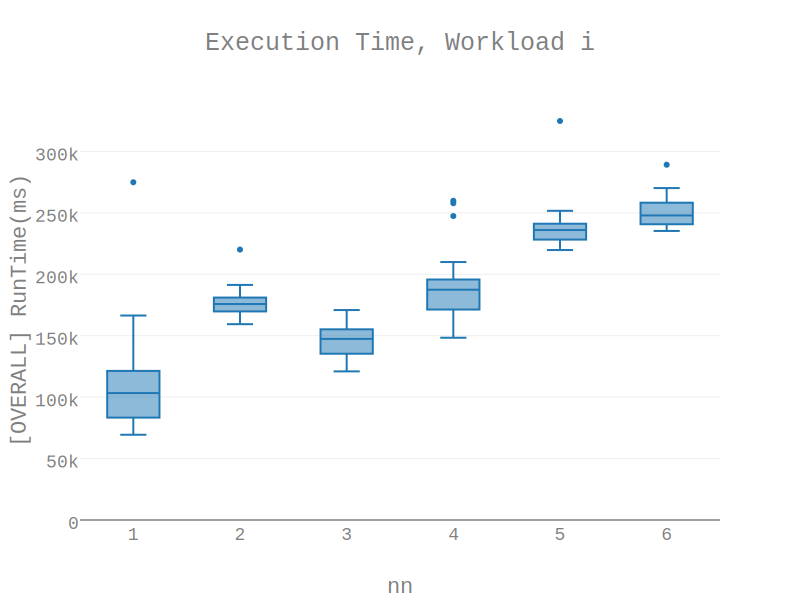
\includegraphics[width=5.5in]{Figures/figures-wli_fig8.pdf}
\caption{}
\label{figures-wli_fig8}
\end{figure}



\subsubsection{Ordinal Statistics}
This section will describe some of the summary statistics that describe the data.  

The summary statistics for Workload I performed on the limited hardware, Raspberry Pi, on the Ethernet local area network are in Table \ref{table:summary_table_i_1GB_rp_wlan}.
\begin{table}
\begin{tabular}{lrrrrrrr}
\toprule
cluster\_size &     1.0 &     2.0 &     3.0 &     4.0 &     5.0 &     6.0 &  Overall \\
\midrule
25\%   & 7.6e+04 & 1.7e+05 & 1.3e+05 & 1.7e+05 & 2.3e+05 & 2.4e+05 &  1.5e+05 \\
50\%   & 8.8e+04 & 1.8e+05 & 1.4e+05 & 1.9e+05 & 2.4e+05 & 2.5e+05 &  1.8e+05 \\
75\%   & 1.2e+05 & 1.8e+05 & 1.5e+05 & 1.9e+05 & 2.4e+05 & 2.6e+05 &  2.4e+05 \\
count &      21 &      21 &      21 &      21 &      21 &      21 &  1.3e+02 \\
max   & 2.7e+05 & 1.9e+05 & 1.6e+05 & 2.6e+05 & 3.2e+05 & 2.9e+05 &  3.2e+05 \\
mean  & 1.1e+05 & 1.8e+05 & 1.4e+05 & 1.9e+05 & 2.4e+05 & 2.5e+05 &  1.8e+05 \\
min   & 6.9e+04 & 1.7e+05 & 1.2e+05 & 1.5e+05 & 2.2e+05 & 2.4e+05 &  6.9e+04 \\
range & 2.1e+05 & 2.4e+04 & 4.3e+04 & 1.1e+05 &   1e+05 & 5.4e+04 &  2.6e+05 \\
std   & 4.7e+04 & 6.1e+03 & 1.4e+04 & 2.3e+04 & 2.1e+04 & 1.3e+04 &  5.7e+04 \\
\bottomrule
\end{tabular}
\caption{Summary Statistics for Workload I performed on a 1GB limited hardware, Raspberry Pi node over a(n)802.11a/b/g/n network.  Except for count, all values are in milliseconds.}
\label{table:summary_table_i_1GB_rp_wlan}
\end{table}



\subsubsection{Analysis}
This section will take a more in-depth look at the data.


\begin{table}[H]
\centering
\begin{tabular}{rrrrr}
\toprule
  slope &  intercept &  r\_value &  p\_value &  std\_err \\
\midrule
2.7e+04 &    8.7e+04 &     0.83 &  3.4e-33 &  1.7e+03 \\
\bottomrule
\end{tabular}
\caption{Linear Regression over Cluster Size, Workload i}
\label{table:wlan_only_i}
\end{table}



\subsection{Wireless Links vs Wired Links}
\subsubsection{Initial Observations}
The results are displayed in Figures \ref{figures-wli_fig7} and \ref{figures-wli_fig9}.  For 1, 2, and 3-node clusters, despite the expected  disparity in execution time, the wired and wireless trends seem to follow each other.  However, from 3 nodes up through 6 nodes, the execution times starts to diverge, suggesting that the wireless has a increasing effect as the number of nodes increases. \begin{figure}[h]
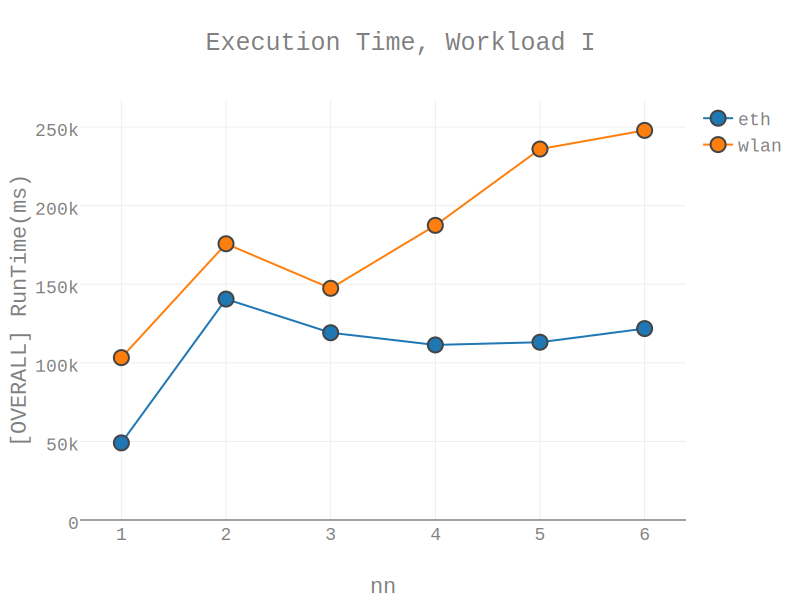
\includegraphics[width=5.5in]{Figures/figures-wli_fig7.pdf}
\caption{}
\label{figures-wli_fig7}
\end{figure}

\begin{figure}[h]
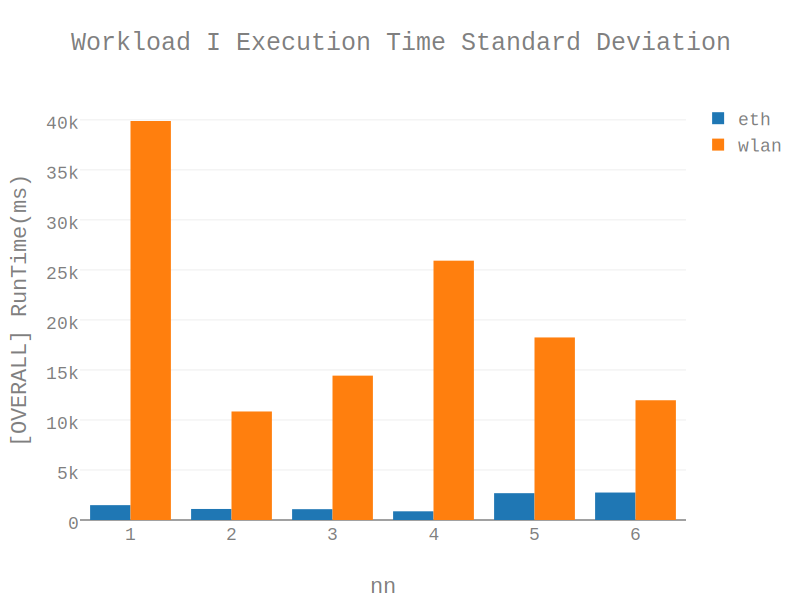
\includegraphics[width=5.5in]{Figures/figures-wli_fig9.pdf}
\caption{}
\label{figures-wli_fig9}
\end{figure}



\subsubsection{Ordinal Statistics}
This section will describe some of the summary statistics that describe the data.  

The summary statistics for Workload I performed on the limited hardware, Raspberry Pi, on the Ethernet local area network are in Table \ref{table:summary_table_i_1GB_rp_eth}.
The summary statistics for Workload I performed on the limited hardware, Raspberry Pi, on the Ethernet local area network are in Table \ref{table:summary_table_i_1GB_rp_wlan}.



\subsubsection{Analysis}
This section will take a more in-depth look at the data.




\begin{table}[H]
\centering
\begin{tabular}{lrrrrr}
\toprule
cluster\_size &   slope &  intercept &  r\_value &  p\_value &  std\_err \\
\midrule
           1 & 5.6e+04 &    4.9e+04 &     0.65 &  2.6e-06 &    1e+04 \\
           2 & 3.7e+04 &    1.4e+05 &     0.97 &    2e-27 &  1.3e+03 \\
           3 & 2.1e+04 &    1.2e+05 &     0.74 &  1.8e-08 &    3e+03 \\
           4 & 7.4e+04 &    1.1e+05 &     0.92 &  9.9e-18 &  5.1e+03 \\
           5 & 1.2e+05 &    1.1e+05 &     0.97 &  3.6e-27 &  4.7e+03 \\
           6 & 1.3e+05 &    1.2e+05 &     0.99 &  1.6e-35 &  2.9e+03 \\
     OVERALL & 7.4e+04 &    1.1e+05 &     0.64 &  3.6e-30 &  5.6e+03 \\
\bottomrule
\end{tabular}
\caption{Linear Regression over the effect of 802.11 links, Workload I}
\label{table:wlan_v_eth_i}
\end{table}





\begin{table}[H]
\centering
\begin{tabular}{llllllll}
\toprule
{} &    0 &    1 &     2 &     3 &    4 &    5 &        6 \\
\midrule
cluster\_size         &    1 &    2 &     3 &     4 &    5 &    6 &  OVERALL \\
ratio\_max\_to\_min     & 0.75 & 0.85 &     1 &  0.76 & 0.52 & 0.53 &      2.1 \\
ratio\_min\_to\_max     & 0.17 & 0.72 &  0.72 &  0.43 & 0.34 & 0.41 &     0.15 \\
ratio\_of\_the\_means   & 0.47 & 0.79 &  0.85 &   0.6 & 0.48 & 0.48 &      0.6 \\
ratio\_of\_the\_medians & 0.56 & 0.79 &  0.84 &   0.6 & 0.48 & 0.49 &     0.66 \\
ratio\_of\_the\_stddevs & 0.02 & 0.19 & 0.071 & 0.033 &  0.1 & 0.16 &     0.51 \\
\bottomrule
\end{tabular}
\caption{Speedup over the effect of 802.11 links, Workload I}
\label{table:wlan_v_eth_i_speedup}
\end{table}





